% Options for packages loaded elsewhere
\PassOptionsToPackage{unicode}{hyperref}
\PassOptionsToPackage{hyphens}{url}
\documentclass[
]{article}
\usepackage{xcolor}
\usepackage{amsmath,amssymb}
\setcounter{secnumdepth}{-\maxdimen} % remove section numbering
\usepackage{iftex}
\ifPDFTeX
  \usepackage[T1]{fontenc}
  \usepackage[utf8]{inputenc}
  \usepackage{textcomp} % provide euro and other symbols
\else % if luatex or xetex
  \usepackage{unicode-math} % this also loads fontspec
  \defaultfontfeatures{Scale=MatchLowercase}
  \defaultfontfeatures[\rmfamily]{Ligatures=TeX,Scale=1}
\fi
\usepackage{lmodern}
\ifPDFTeX\else
  % xetex/luatex font selection
\fi
% Use upquote if available, for straight quotes in verbatim environments
\IfFileExists{upquote.sty}{\usepackage{upquote}}{}
\IfFileExists{microtype.sty}{% use microtype if available
  \usepackage[]{microtype}
  \UseMicrotypeSet[protrusion]{basicmath} % disable protrusion for tt fonts
}{}
\makeatletter
\@ifundefined{KOMAClassName}{% if non-KOMA class
  \IfFileExists{parskip.sty}{%
    \usepackage{parskip}
  }{% else
    \setlength{\parindent}{0pt}
    \setlength{\parskip}{6pt plus 2pt minus 1pt}}
}{% if KOMA class
  \KOMAoptions{parskip=half}}
\makeatother
\usepackage{listings}
\newcommand{\passthrough}[1]{#1}
\lstset{defaultdialect=[5.3]Lua}
\lstset{defaultdialect=[x86masm]Assembler}
\usepackage{longtable,booktabs,array}
\newcounter{none} % for unnumbered tables
\usepackage{calc} % for calculating minipage widths
% Correct order of tables after \paragraph or \subparagraph
\usepackage{etoolbox}
\makeatletter
\patchcmd\longtable{\par}{\if@noskipsec\mbox{}\fi\par}{}{}
\makeatother
% Allow footnotes in longtable head/foot
\IfFileExists{footnotehyper.sty}{\usepackage{footnotehyper}}{\usepackage{footnote}}
\makesavenoteenv{longtable}
% definitions for citeproc citations
\NewDocumentCommand\citeproctext{}{}
\NewDocumentCommand\citeproc{mm}{%
  \begingroup\def\citeproctext{#2}\cite{#1}\endgroup}
\makeatletter
 % allow citations to break across lines
 \let\@cite@ofmt\@firstofone
 % avoid brackets around text for \cite:
 \def\@biblabel#1{}
 \def\@cite#1#2{{#1\if@tempswa , #2\fi}}
\makeatother
\newlength{\cslhangindent}
\setlength{\cslhangindent}{1.5em}
\newlength{\csllabelwidth}
\setlength{\csllabelwidth}{3em}
\newenvironment{CSLReferences}[2] % #1 hanging-indent, #2 entry-spacing
 {\begin{list}{}{%
  \setlength{\itemindent}{0pt}
  \setlength{\leftmargin}{0pt}
  \setlength{\parsep}{0pt}
  % turn on hanging indent if param 1 is 1
  \ifodd #1
   \setlength{\leftmargin}{\cslhangindent}
   \setlength{\itemindent}{-1\cslhangindent}
  \fi
  % set entry spacing
  \setlength{\itemsep}{#2\baselineskip}}}
 {\end{list}}
\usepackage{calc}
\newcommand{\CSLBlock}[1]{\hfill\break\parbox[t]{\linewidth}{\strut\ignorespaces#1\strut}}
\newcommand{\CSLLeftMargin}[1]{\parbox[t]{\csllabelwidth}{\strut#1\strut}}
\newcommand{\CSLRightInline}[1]{\parbox[t]{\linewidth - \csllabelwidth}{\strut#1\strut}}
\newcommand{\CSLIndent}[1]{\hspace{\cslhangindent}#1}
\setlength{\emergencystretch}{3em} % prevent overfull lines
\providecommand{\tightlist}{%
  \setlength{\itemsep}{0pt}\setlength{\parskip}{0pt}}
% whitepaper/latex/header.tex
%
% Preamble fragment injected into pandoc's default LaTeX template via
% `--include-in-header`. Loads the arXiv preprint style and the
% packages we need for code, tables, math, and Unicode glyphs that
% appear in Aether's typing rules (Γ, ⊢, ↦, ⊥, etc.).
%
% Compiled with Tectonic (XeTeX backend); fontspec / unicode-math are
% the right path for Unicode glyphs in body text. pdflatex would need
% manual `\DeclareUnicodeCharacter` declarations.

\usepackage{arxiv}

\usepackage{amsmath,amssymb}

% Pandoc's default LaTeX template already loads `unicode-math` (which
% pulls in `fontspec`) when the engine is XeTeX/LuaTeX. We deliberately
% do NOT call `\setmainfont`/`\setsansfont` here: by name, "Latin Modern
% Roman" is not a Windows or macOS system font, and Tectonic's font
% lookup goes through the OS font directory before its bundled TeX Live
% tree. Letting XeTeX fall back to its default font (Computer
% Modern / Latin Modern via NFSS) keeps the build host-agnostic.
% arxiv.sty's `\renewcommand{\rmdefault}{ptm}` etc. then take effect.

% Code listings (pandoc --listings).
\usepackage{listings}
\usepackage{xcolor}
\lstset{
  basicstyle=\ttfamily\small,
  breaklines=true,
  breakatwhitespace=false,
  columns=fullflexible,
  keepspaces=true,
  showstringspaces=false,
  frame=single,
  framesep=4pt,
  rulecolor=\color{gray!50},
  backgroundcolor=\color{gray!5},
  extendedchars=true,
  inputencoding=utf8,
  literate=
    {Γ}{{$\Gamma$}}1
    {⊢}{{$\vdash$}}1
    {↦}{{$\mapsto$}}1
    {⊥}{{$\bot$}}1
    {α}{{$\alpha$}}1
    {β}{{$\beta$}}1
    {γ}{{$\gamma$}}1
    {τ}{{$\tau$}}1
    {ε}{{$\varepsilon$}}1
    {≤}{{$\leq$}}1
    {≥}{{$\geq$}}1
    {≠}{{$\neq$}}1
    {→}{{$\rightarrow$}}1
    {←}{{$\leftarrow$}}1
    {∈}{{$\in$}}1
    {∉}{{$\notin$}}1
    {∀}{{$\forall$}}1
    {∃}{{$\exists$}}1
    {⊕}{{$\oplus$}}1
    {…}{{\ldots}}1
    {–}{{--}}1
    {—}{{---}}1
    {×}{{$\times$}}1
    {≈}{{$\approx$}}1
    {─}{{\textendash\textendash}}1
    {│}{{|}}1
    {├}{{|--}}1
    {└}{{`--}}1
    {┌}{{,--}}1
    {┐}{{--.}}1
    {┘}{{--'}}1
    {╴}{{--}}1
    {╶}{{--}}1
    {⌈}{{$\lceil$}}1
    {⌉}{{$\rceil$}}1
    {⌊}{{$\lfloor$}}1
    {⌋}{{$\rfloor$}}1
    {¬}{{$\neg$}}1
    {∨}{{$\vee$}}1
    {∧}{{$\wedge$}}1,
}

% Wide tables.
\usepackage{longtable}
\usepackage{booktabs}

% Figures generated by bench/figures/generate_figures.py into latex/figures/.
% Tectonic runs from whitepaper/latex/, so the relative path resolves directly.
\usepackage{graphicx}
\graphicspath{{figures/}}

% Hyperlinks; load near the end of the preamble.
\usepackage[hidelinks,unicode=true]{hyperref}
\usepackage{microtype}

% Tighter table column padding so the wide reproducibility table fits.
\setlength{\tabcolsep}{4pt}

% Allow long URLs to break.
\usepackage{xurl}
\usepackage{bookmark}
\IfFileExists{xurl.sty}{\usepackage{xurl}}{} % add URL line breaks if available
\urlstyle{same}
\hypersetup{
  pdftitle={Aether: A Domain-Specific Language for Type-Safe LLM Orchestration},
  pdfauthor={Md. Sowad Al-Mughni},
  hidelinks,
  pdfcreator={LaTeX via pandoc}}

\title{Aether: A Domain-Specific Language for Type-Safe LLM
Orchestration}
\author{Md. Sowad Al-Mughni}
\date{May 2026}

\begin{document}
\maketitle

\subsection{Abstract}\label{abstract}

Large language model (LLM) integration in production systems suffers
from five systematic engineering failures: runtime-only type checking,
complex workflow orchestration without static validation, inadequate
testing methodologies, suboptimal caching, and insufficient security
guarantees. Existing tools address these problems in isolation:
orchestration frameworks provide flexibility without compile-time
safety, typed output libraries focus narrowly on schema validation, and
security tools operate only at runtime.

This paper presents Aether, a domain-specific language that treats LLM
orchestration as a first-class engineering discipline. Aether introduces
three core abstractions: \passthrough{\lstinline!llm fn!} for typed LLM
interactions, \passthrough{\lstinline!flow!} for DAG-based workflow
composition, and \passthrough{\lstinline!context!} for state management.
The Aether compiler performs static analysis to verify type contracts
across workflow steps, identify parallelization opportunities, and
enforce security policies through compile-time taint tracking.

We make five contributions: (1) a type system spanning LLM inputs,
outputs, and workflow compositions with compile-time verification; (2) a
DAG-based intermediate representation enabling static optimization; (3)
a reproducible benchmark methodology for LLM orchestration systems with
full JSON artifacts under \passthrough{\lstinline!bench/results/!}; (4)
an open-source prototype implementation with \textbf{OTLP tracing}
(OpenTelemetry 0.21.0) and \textbf{Criterion benchmarks}; and (5)
compile-time taint tracking with measured \textbf{100\% catch rate} on a
60-case adapted InjecAgent corpus, validating that prompt-injection
defense can be enforced before any LLM call (Section 9.8,
\passthrough{\lstinline!bench/results/security\_v1.json!}). Measured
outcomes: parallel execution yields a paired BCa speedup of
\textbf{1.4778×} on \passthrough{\lstinline!customer\_support\_100!} and
\textbf{2.5841×} on \passthrough{\lstinline!document\_analysis\_50!}
(\passthrough{\lstinline!bench/results/ablation\_parallel\_v1.json!});
the L1 exact-match cache reaches a hit rate of \textbf{0.7000} on a
70\%-repeat workload and \textbf{1.0000} under warm-cache
(\passthrough{\lstinline!bench/results/ablation\_cache\_v1.json!}); the
compiler catches \textbf{30 of 30} intentionally malformed programs at
compile time, vs \textbf{17 of 30} caught at runtime by LangChain and
DSPy, with \textbf{13 missed silently} by each baseline
(\passthrough{\lstinline!bench/results/ablation\_typesafety\_v1.json!}).
The end-to-end real-OpenAI run (3 trials, both datasets, all three
systems) is in
\passthrough{\lstinline!bench/results/real\_api\_v1.json!} (Aether cost
\$0.128887, \$0.478349 total).

\textbf{Keywords}: domain-specific languages, large language models,
type systems, workflow orchestration, static analysis

\begin{quote}
\textbf{Reproducibility.} Every numeric claim in this paper is traceable
to a JSON file in \passthrough{\lstinline!bench/results/!} produced by a
specific run. The full inventory:

{\def\LTcaptype{none} % do not increment counter
\begin{longtable}[]{@{}
  >{\raggedright\arraybackslash}p{(\linewidth - 10\tabcolsep) * \real{0.1579}}
  >{\raggedright\arraybackslash}p{(\linewidth - 10\tabcolsep) * \real{0.1579}}
  >{\raggedright\arraybackslash}p{(\linewidth - 10\tabcolsep) * \real{0.1579}}
  >{\raggedright\arraybackslash}p{(\linewidth - 10\tabcolsep) * \real{0.1579}}
  >{\raggedleft\arraybackslash}p{(\linewidth - 10\tabcolsep) * \real{0.2105}}
  >{\raggedright\arraybackslash}p{(\linewidth - 10\tabcolsep) * \real{0.1579}}@{}}
\toprule\noalign{}
\begin{minipage}[b]{\linewidth}\raggedright
File
\end{minipage} & \begin{minipage}[b]{\linewidth}\raggedright
git\_version (or library)
\end{minipage} & \begin{minipage}[b]{\linewidth}\raggedright
Provider
\end{minipage} & \begin{minipage}[b]{\linewidth}\raggedright
Scope
\end{minipage} & \begin{minipage}[b]{\linewidth}\raggedleft
Trials
\end{minipage} & \begin{minipage}[b]{\linewidth}\raggedright
\passthrough{\lstinline!measured\_at!}
\end{minipage} \\
\midrule\noalign{}
\endhead
\bottomrule\noalign{}
\endlastfoot
\passthrough{\lstinline!bench/results/aether\_mock\_v1.json!} &
\passthrough{\lstinline!4d16ec5cd5cb0957d7dc6408b5df25ba7befbe9b!} &
mock & customer\_support\_100 + document\_analysis\_50; sequential /
parallel / parallel\_cached & 5 & 2026-05-03T09:49:57Z \\
\passthrough{\lstinline!bench/results/langchain\_v1.json!} &
\passthrough{\lstinline!9591852f9ebb34822dc628197d47cb643c0ac381!}
(langchain 0.3.28) & mock & same & 5 & 2026-05-04T05:18:25Z \\
\passthrough{\lstinline!bench/results/dspy\_v1.json!} &
\passthrough{\lstinline!558df452e1e9c36d35bdbc474369862a631c458c!} (dspy
2.6.27) & mock & same & 5 & 2026-05-08T02:37:56Z \\
\passthrough{\lstinline!bench/results/aether\_real\_api\_v1.json!} &
\passthrough{\lstinline!9c8001ce269920c98fa733a82b3c69ea7352e37e!} &
openai (gpt-4o-mini) & same & 3 & 2026-05-08T06:29:58Z \\
\passthrough{\lstinline!bench/results/langchain\_real\_api\_v1.json!} &
langchain 0.3.28 & openai & same & 3 & 2026-05-08 \\
\passthrough{\lstinline!bench/results/dspy\_real\_api\_v1.json!} & dspy
2.6.27 & openai & same & 3 & 2026-05-08 \\
\passthrough{\lstinline!bench/results/real\_api\_v1.json!} & merged &
openai & both datasets, all 3 systems, end-to-end cost & --- &
2026-05-08T09:26:39Z \\
\passthrough{\lstinline!bench/results/ablation\_cache\_v1.json!} &
\passthrough{\lstinline!8aee2cce5f969b5e2d84e94216355354dcc0eb7f!} &
mock & customer\_support\_100 + customer\_support\_repeat\_100;
no\_cache / l1\_exact\_match / repeat\_warm & 5 &
2026-05-08T13:05:22Z \\
\passthrough{\lstinline!bench/results/ablation\_parallel\_v1.json!} &
\passthrough{\lstinline!8aee2cce5f969b5e2d84e94216355354dcc0eb7f!} &
mock & customer\_support\_100 + document\_analysis\_50; sequential vs
parallel; paired BCa speedup & 5 & 2026-05-08T13:09:48Z \\
\passthrough{\lstinline!bench/results/ablation\_typesafety\_v1.json!} &
\passthrough{\lstinline!8aee2cce5f969b5e2d84e94216355354dcc0eb7f!} & n/a
(compile-time + mock LLM) & 30-case error-injection corpus across 4
buckets & n/a & 2026-05-08T13:15:35Z \\
\passthrough{\lstinline!bench/results/security\_v1.json!} &
\passthrough{\lstinline!2759f1e7f5e26eb435f3c98951ea1fcf193f2b5e!} &
openai (gpt-4o-mini) & InjecAgent-adapted, 20 attack + 20 benign cases ×
3 trials × 3 configs & 3 & 2026-05-08T18:41:38Z \\
\passthrough{\lstinline!bench/results/hotpotqa\_aether\_v1.json!} &
\passthrough{\lstinline!b581653a0611fdc3ddfbaf8af9553593a61cb585!} &
mock & hotpotqa\_dev\_500 (latency only; mock LLM does not produce real
answers) & 3 & 2026-05-08T10:09:11Z \\
\passthrough{\lstinline!bench/results/hotpotqa\_langchain\_v1.json!} &
\passthrough{\lstinline!b581653a0611fdc3ddfbaf8af9553593a61cb585!} &
mock & same & 3 & 2026-05-08T10:12:13Z \\
\passthrough{\lstinline!bench/results/hotpotqa\_dspy\_v1.json!} &
\passthrough{\lstinline!b581653a0611fdc3ddfbaf8af9553593a61cb585!} &
mock & same & 3 & 2026-05-08 \\
\end{longtable}
}

Reproduction: clone the repo at the listed commit, install
\passthrough{\lstinline!aether-runtime!} with the
\passthrough{\lstinline!llm-api!} feature for real-API runs, and invoke
\passthrough{\lstinline!scripts/run\_benchmark.py!} (mock) or
\passthrough{\lstinline!scripts/run\_real\_api\_benchmark.sh!} (OpenAI)
per Section 13. Markdown summaries of the real-API run and the ablation
suite are at \passthrough{\lstinline!bench/results/REAL\_API.md!} and
\passthrough{\lstinline!bench/results/ablations\_v1.md!}.
\end{quote}

\subsection{1. Introduction}\label{introduction}

Large language models are increasingly deployed in production systems,
yet the engineering practices for integrating them remain ad hoc.
Developers face fragile prompt chains, unpredictable outputs, absent
testing methodologies, and significant operational costs. Existing
solutions address these problems piecemeal: orchestration frameworks
like LangChain provide flexibility without compile-time safety, while
typed output libraries like BAML focus narrowly on schema validation.

Aether is a domain-specific programming language designed to treat LLM
orchestration as a first-class engineering discipline. The language
introduces three core abstractions: \passthrough{\lstinline!llm fn!} for
typed LLM interactions with explicit input/output schemas,
\passthrough{\lstinline!flow!} for DAG-based workflow orchestration, and
\passthrough{\lstinline!context!} for state management across
interactions. The Aether compiler performs static analysis to verify
type contracts, identify parallelization opportunities, and generate
optimized execution plans.

\textbf{Current Status}: Aether is a working prototype. The compiler
(lexer, parser, 5-pass semantic analyzer, DAG code generator) and
runtime (parallel execution, LRU caching, multi-provider support) are
implemented. The benchmark infrastructure is complete with synthetic
datasets and CI integration. All performance claims in this paper are
validated against this implementation; Section 9 reports empirical
results. Detailed implementation status is in Appendix B.

\subsubsection{1.1 Contributions}\label{contributions}

This paper makes the following contributions:

\begin{enumerate}
\def\labelenumi{\arabic{enumi}.}
\item
  \textbf{Type System for LLM Orchestration} (Section 5): A static type
  system that spans LLM inputs, outputs, and workflow compositions,
  enabling compile-time verification of type contracts across workflow
  steps.
\item
  \textbf{DAG-Based Intermediate Representation} (Section 6): A compiler
  architecture that transforms Aether source into a directed acyclic
  graph representation, enabling static identification of
  parallelization opportunities and dependency-aware scheduling.
\item
  \textbf{Reproducible Evaluation Methodology} (Section 8): A benchmark
  suite design with synthetic datasets, baseline implementations, and
  ablation study infrastructure for fair comparison of LLM orchestration
  approaches.
\item
  \textbf{Open-Source Prototype} (Section 13): A working implementation
  comprising a compiler (lexer, parser, semantic analyzer, code
  generator) and runtime (parallel execution, caching, observability),
  demonstrating feasibility of the approach. The runtime was executed
  end-to-end against the real OpenAI API (Section 9.6.5) and results are
  committed in
  \passthrough{\lstinline!bench/results/real\_api\_v1.json!}.
\item
  \textbf{Compile-Time Taint Tracking with Measured Effectiveness}
  (Sections 9.8, 11): A static taint analysis that distinguishes trusted
  from untrusted prompt fragments, with a measured 100\% compile-time
  catch rate (CI degenerate) on a 60-case InjecAgent-adapted corpus run
  against \passthrough{\lstinline!gpt-4o-mini!}
  (\passthrough{\lstinline!bench/results/security\_v1.json!}). Aether
  blocks the malicious \emph{program shape} statically, before any LLM
  call is issued.
\end{enumerate}

\subsection{2. Problem Statement and
Motivation}\label{problem-statement-and-motivation}

The integration of LLMs into production software exhibits systematic
engineering failures that current tools address incompletely.

\subsubsection{2.1 The Type Safety Gap}\label{the-type-safety-gap}

LLM APIs accept strings and return strings. The semantic structure
within those strings (JSON schemas, enumerated values, structured
responses) exists only as informal contracts enforced at runtime. When
an LLM returns malformed output, the error surfaces far from its source.
DSPy (Khattab et al. 2024) introduced typed signatures but remains
embedded in Python's dynamic type system. BAML (Boundary ML 2024)
generates typed clients but does not extend type checking to workflow
composition. Neither provides compile-time verification that a sequence
of LLM calls produces type-compatible results.

\textbf{Measurable problem}: In production systems using LangChain,
schema validation failures occur at runtime, requiring defensive
programming patterns that increase code complexity by an estimated
20-40\% (based on manual code review of open-source projects).

\subsubsection{2.2 The Orchestration Complexity
Problem}\label{the-orchestration-complexity-problem}

Multi-step LLM workflows involve conditional routing, parallel
execution, error handling, and state management. LangChain's LCEL
provides composability but offers no static guarantees about workflow
validity. LangGraph 1.0 (LangChain Inc. 2025) introduced durable state
management but relies on runtime graph construction. Temporal (Temporal
Technologies 2023) provides robust workflow orchestration but treats LLM
calls as opaque activities without domain-specific optimization.

\textbf{Measurable problem}: Workflow errors (unreachable nodes, type
mismatches between steps, missing error handlers) are detected only at
runtime, extending debugging cycles.

\subsubsection{2.3 The Testing Deficit}\label{the-testing-deficit}

LLM outputs are probabilistic, making traditional unit testing
insufficient. Evaluation frameworks like DeepEval (Confident AI 2024)
and LangSmith (LangChain Inc. 2024) provide runtime testing
capabilities, but test definitions remain separate from application
code. There is no compile-time verification that test assertions match
declared output schemas or that evaluation metrics are applicable to
specific LLM function signatures.

\textbf{Measurable problem}: Test coverage for LLM applications is
typically lower than for traditional software because testing
infrastructure is bolted on rather than integrated ({Chen et al.} 2021).

\subsubsection{2.4 The Cost and Latency
Challenge}\label{the-cost-and-latency-challenge}

LLM API calls incur latency (hundreds of milliseconds to seconds) and
monetary cost. Provider-level prompt caching (Anthropic: 90\% cost
reduction (Anthropic 2024b); OpenAI: 50\% discount (OpenAI 2024))
requires specific prompt structures that are difficult to maintain
manually. Semantic caching libraries like GPTCache have seen reduced
maintenance, with the project noting it no longer supports new APIs
(Zilliz 2024).

\textbf{Measurable problem}: Organizations report 30-60\% of LLM API
spend could be eliminated with better caching, but implementing caching
correctly requires understanding prompt structure at the application
level.

\subsubsection{2.5 The Security Surface}\label{the-security-surface}

Prompt injection remains the top risk in OWASP's LLM Top 10 (2025)
(OWASP 2025). Runtime guardrails show limited effectiveness:
instructional defenses achieve only approximately 70\% attack success
reduction, while delimiter isolation provides minimal protection
(approximately 85\% attack success rate) ({Liu et al.} 2023).
Training-time defenses like StruQ achieve 0\% attack success rate
({Jatmo et al.} 2024), but application-level defenses remain critical
for deployed systems.

\textbf{Measurable problem}: No existing framework provides compile-time
verification that untrusted input is properly isolated from system
prompts across an entire workflow.

\subsubsection{2.6 Why a Language-Level
Approach}\label{why-a-language-level-approach}

These problems share a common root: LLM integration occurs at runtime,
in strings, without static verification. A domain-specific language can
address this by moving verification earlier, enabling whole-program
analysis, and integrating cross-cutting concerns as language features.

This approach has precedent: SQL moved database queries from string
manipulation to a typed query language, enabling query optimization and
type checking. Aether aims to do the same for LLM interactions.

\subsubsection{2.7 Research Hypotheses}\label{research-hypotheses}

Based on the problems identified above, we formulate three testable
hypotheses:

\textbf{H1 (Type Safety)}: Compile-time type checking reduces runtime
schema and type failures by at least 80\% compared to runtime-only
validation approaches (LangChain, raw API calls).

\textbf{H2 (Latency)}: DAG-based scheduling reduces end-to-end latency
by at least 30\% on workflows with parallelizable LLM calls compared to
sequential execution.

\textbf{H3 (Cost Efficiency)}: Compiler-assisted prompt structuring
increases cache hit rates by at least 40\% compared to manual caching
implementations.

These hypotheses correspond to success criteria SC-1, SC-4, and SC-5
respectively. Section 9 presents empirical evaluation of each
hypothesis.

\subsection{3. Related Work}\label{related-work}

This section surveys the LLM integration landscape as of early 2026,
positioning Aether within the existing ecosystem. We acknowledge both
the strengths of existing approaches and areas where Aether's design
remains unproven.

\subsubsection{3.1 Orchestration
Frameworks}\label{orchestration-frameworks}

\textbf{LangChain/LangGraph} (LangChain Inc. 2025): LangChain 1.0
(October 2025) shifted from explicit LCEL pipe operators to a
middleware-based architecture. LangGraph 1.0 introduced durable state
management enabling agent execution to persist through failures.
Strengths include a large ecosystem and production deployment
experience. Limitations include runtime-only type checking and no
compile-time workflow validation.

\textbf{DSPy} (Khattab et al. 2024): The most conceptually aligned
existing approach. DSPy (Stanford, ICLR 2024 Spotlight) treats prompts
as declarative signatures with typed inputs and outputs. A compiler
automatically optimizes prompts and few-shot examples, demonstrating
25-65\% improvement over standard few-shot approaches. Limitation:
remains embedded in Python without static cross-module type checking.

\textbf{LlamaIndex Workflows} (LlamaIndex Inc. 2025): Workflows 1.0
(June 2025) provides event-driven, async-first execution with stateful
pause/resume. Strong for RAG applications but limited workflow
orchestration primitives.

\textbf{CrewAI} (CrewAI Inc. 2025): Distinguishes between Crews
(role-based autonomous collaboration) and Flows (deterministic
event-driven workflows). Claims 5.76x performance improvement over
LangGraph in certain benchmarks, though methodology is not independently
verified.

\subsubsection{3.2 Typed Output Libraries}\label{typed-output-libraries}

\textbf{BAML} (Boundary ML 2024): A domain-specific language providing
compile-time type generation for prompts. Key features include 60\%
fewer tokens than JSON Schema, type-safe streaming, and full LSP
tooling. BAML validates the compile-time DSL approach with production
adoption. Limitation: focuses on structured outputs without workflow
orchestration or caching.

\textbf{Instructor} (Liu 2024): Wraps provider SDKs with Pydantic model
integration and automatic retries (3M+ monthly downloads). Runtime-only
type enforcement.

\textbf{Outlines} ({.txt} 2024): Compiles JSON Schema to finite state
machines for constrained decoding, achieving 100\% structural validity.
Runtime compilation, not integrated with workflow orchestration.

\textbf{Provider APIs}: OpenAI and Anthropic offer structured output
modes with 100\% schema compliance through constrained decoding
{[}Anthropic (2024b){]}(OpenAI 2024). Limited to single calls without
cross-call type verification.

\subsubsection{3.3 Evaluation Frameworks}\label{evaluation-frameworks}

\textbf{LangSmith} (LangChain Inc. 2024): End-to-end observability with
tracing, online evaluations, and LLM-as-judge evaluators. Multi-turn
evaluation support launched 2025.

\textbf{DeepEval} (Confident AI 2024): Pytest-style unit testing with
50+ built-in metrics including G-Eval and RAG metrics. Version 3.0 added
component-level evaluation.

\textbf{RAGAS} (Es et al. 2024): Reference-free RAG evaluation (EACL
2024) with metrics for faithfulness, answer relevancy, and context
precision.

\subsubsection{3.4 Workflow Engines}\label{workflow-engines}

\textbf{Temporal} (Temporal Technologies 2023): Provides durable
execution through event sourcing, automatic retries, and exactly-once
semantics. OpenAI Agents SDK integration announced 2025. Requires manual
determinism discipline; no LLM-specific primitives.

\textbf{Prefect 3.0} (Prefect Technologies 2024): Transactional
semantics with 90\%+ overhead reduction. ControlFlow framework provides
agentic workflows with Pydantic AI integration.

\subsubsection{3.5 Security Tools}\label{security-tools}

\textbf{Guardrails AI} (Guardrails AI 2024): Composable validators with
configurable on-fail actions. Runtime-only enforcement.

\textbf{NeMo Guardrails} (NVIDIA 2024): Colang DSL for declarative
guardrail definitions. Addresses runtime guardrails but not compile-time
verification.

\textbf{StruQ} ({Jatmo et al.} 2024): Training-time defense achieving
0\% attack success rate through structured query separation.
Demonstrates that architectural approaches outperform runtime
guardrails.

\subsubsection{3.6 Interoperability
Protocols}\label{interoperability-protocols}

\textbf{MCP (Model Context Protocol)} (Anthropic 2024a): Anthropic's
standard (November 2024) for agent-tool integration using JSON-RPC 2.0.
Adopted by OpenAI and Google DeepMind in early 2025.

\textbf{A2A (Agent-to-Agent Protocol)} (Google 2025): Google's standard
(April 2025, now Linux Foundation) for agent-to-agent communication.
150+ partner organizations.

\subsubsection{3.7 Comparative Analysis}\label{comparative-analysis}

{\def\LTcaptype{none} % do not increment counter
\begin{longtable}[]{@{}
  >{\raggedright\arraybackslash}p{(\linewidth - 10\tabcolsep) * \real{0.1633}}
  >{\raggedright\arraybackslash}p{(\linewidth - 10\tabcolsep) * \real{0.2245}}
  >{\raggedright\arraybackslash}p{(\linewidth - 10\tabcolsep) * \real{0.1224}}
  >{\raggedright\arraybackslash}p{(\linewidth - 10\tabcolsep) * \real{0.1224}}
  >{\raggedright\arraybackslash}p{(\linewidth - 10\tabcolsep) * \real{0.2041}}
  >{\raggedright\arraybackslash}p{(\linewidth - 10\tabcolsep) * \real{0.1633}}@{}}
\toprule\noalign{}
\begin{minipage}[b]{\linewidth}\raggedright
Aspect
\end{minipage} & \begin{minipage}[b]{\linewidth}\raggedright
LangChain
\end{minipage} & \begin{minipage}[b]{\linewidth}\raggedright
DSPy
\end{minipage} & \begin{minipage}[b]{\linewidth}\raggedright
BAML
\end{minipage} & \begin{minipage}[b]{\linewidth}\raggedright
Temporal
\end{minipage} & \begin{minipage}[b]{\linewidth}\raggedright
Aether
\end{minipage} \\
\midrule\noalign{}
\endhead
\bottomrule\noalign{}
\endlastfoot
Abstraction & Library & Compiler & DSL & Workflow Engine & Full DSL \\
Type Safety & Runtime & Runtime (typed sigs) & Compile-time (output) &
None (LLM) & Compile-time (I/O + flow) \\
Workflow Orchestration & Chain/Graph & Module composition & None & DAG &
DAG \\
Caching & External & None & None & None & Integrated \\
Evaluation & External (LangSmith) & Built-in metrics & None & None &
Language-level (planned) \\
Security & External & None & None & None & Compile-time taint
(planned) \\
Observability & Built-in & Limited & None & Built-in & Integrated \\
Durable Execution & LangGraph & None & None & Native & Compilation
target (planned) \\
\end{longtable}
}

\textbf{Honest Assessment}: Aether proposes to unify capabilities that
exist separately in mature tools. The value proposition depends on
whether compile-time verification provides sufficient benefit over
runtime approaches to justify learning a new language. This remains to
be validated empirically.

\subsection{4. Design Goals and Measurable Success
Criteria}\label{design-goals-and-measurable-success-criteria}

Aether's design is guided by five principles, each with measurable
success criteria that will determine whether the language achieves its
goals.

\subsubsection{4.1 Reliability Through Type
Safety}\label{reliability-through-type-safety}

\textbf{Goal}: Catch LLM integration errors at compile time rather than
runtime.

\textbf{Design Approach}: - Strong static typing for LLM inputs and
outputs with inference across workflow steps - Compile-time verification
that LLM function compositions are type-compatible - Runtime fallback
with typed error handling for LLM output deviations

\textbf{Success Criteria} (evaluated in Section 9.5): - SC-1: Reduce
runtime type errors by \textgreater80\% compared to equivalent LangChain
implementations - SC-2: Achieve \textless5\% false positive rate for
compile-time type errors - SC-3: Maintain \textless10\% compile time
overhead compared to Python type checking (mypy)

\textbf{Current Status}: Type system implemented for LLM function
validation (model/prompt required), symbol resolution, and basic type
collection. Full cross-flow type inference in progress.

\subsubsection{4.2 Efficiency Through Static
Optimization}\label{efficiency-through-static-optimization}

\textbf{Goal}: Reduce latency and cost through compiler-driven
optimization.

\textbf{Design Approach}: - DAG-based intermediate representation
enabling parallelization - Compiler-generated caching strategies based
on prompt structure analysis - Static identification of batching
opportunities

\textbf{Success Criteria} (evaluated in Sections 9.2 and 9.3): - SC-4:
Achieve \textgreater30\% latency reduction on parallelizable workflows
compared to sequential execution - SC-5: Achieve \textgreater40\% cache
hit rate improvement through compiler-assisted prompt structuring -
SC-6: Reduce API costs by \textgreater25\% on representative benchmarks
through batching and caching

\textbf{Current Status}: Runtime implements level-based parallel
execution (JoinSet) and exact-match LRU caching. Benchmark
infrastructure is complete with synthetic datasets, Python benchmark
runner, provider switching, and CI integration. See Section 8 for
methodology and Section 9 for results.

\subsubsection{4.3 Modularity Through
Composition}\label{modularity-through-composition}

\textbf{Goal}: Enable reusable LLM components with clear interfaces.

\textbf{Design Approach}: - \passthrough{\lstinline!llm fn!} as
composable units with explicit signatures -
\passthrough{\lstinline!flow!} as declarative workflow definitions -
\passthrough{\lstinline!context!} as first-class state management

\textbf{Success Criteria}: - SC-7: Achieve \textgreater90\% code reuse
rate for common LLM patterns across projects - SC-8: Reduce lines of
code by \textgreater30\% compared to equivalent Python implementations

\textbf{Current Status}: Syntax fully implemented, parser complete.
Semantic analysis tracks \passthrough{\lstinline!llm fn!},
\passthrough{\lstinline!flow!}, \passthrough{\lstinline!struct!}, and
\passthrough{\lstinline!enum!} definitions. Success criteria measurable
after tooling ecosystem is complete.

\subsubsection{4.4 Testability Through Language
Integration}\label{testability-through-language-integration}

\textbf{Goal}: Make LLM testing a first-class language concern.

\textbf{Design Approach}: - Built-in \passthrough{\lstinline!test!}
blocks with typed assertions - Golden dataset integration with schema
alignment verification - Compile-time validation that test assertions
match declared output schemas

\textbf{Success Criteria}: - SC-9: Increase test coverage on LLM
applications by \textgreater50\% compared to baseline - SC-10: Reduce
test maintenance burden by \textgreater40\% through schema-test
alignment

\textbf{Current Status}: Test block syntax designed, parser support
incomplete.

\subsubsection{4.5 Security Through Compile-Time
Verification}\label{security-through-compile-time-verification}

\textbf{Goal}: Provide security guarantees beyond runtime guardrails.

\textbf{Design Approach}: - Taint tracking distinguishing trusted system
prompts from untrusted user input - Compile-time verification of
guardrail presence - Static analysis of tool access permissions

\textbf{Success Criteria}: - SC-11: Catch \textgreater90\% of prompt
injection vulnerabilities that pass runtime guardrails in static
analysis - SC-12: Zero false negatives for taint tracking violations

\textbf{Current Status}: Security model designed, not yet implemented.
Success criteria derived from StruQ research showing architectural
approaches outperform runtime guardrails.

\subsection{5. Language Design}\label{language-design}

Aether is a statically-typed, domain-specific language for LLM
orchestration. This section presents the core abstractions and their
semantics. The formal grammar is provided in Appendix A.

\subsubsection{5.1 Core Abstractions}\label{core-abstractions}

\paragraph{\texorpdfstring{5.1.1 LLM Functions
(\texttt{llm\ fn})}{5.1.1 LLM Functions (llm fn)}}\label{llm-functions-llm-fn}

An \passthrough{\lstinline!llm fn!} encapsulates a single LLM
interaction with explicit type contracts:

\begin{lstlisting}
llm fn classify_sentiment(text: string) -> Sentiment {
    model: "gpt-4o",
    temperature: 0.1,
    prompt: "Classify the sentiment of the following text as Positive, Neutral, or Negative.

Text: {{text}}

Respond with only the sentiment classification."
}

enum Sentiment { Positive, Neutral, Negative }
\end{lstlisting}

\textbf{Semantics}: - Input parameters are type-checked at compile time
- The output type constrains the expected LLM response - The compiler
generates parsing and validation code for the output type - Runtime
\passthrough{\lstinline!ParseError!} is raised if the LLM output does
not conform to the schema

\paragraph{\texorpdfstring{5.1.2 Flows
(\texttt{flow})}{5.1.2 Flows (flow)}}\label{flows-flow}

A \passthrough{\lstinline!flow!} defines an orchestrated workflow as a
directed acyclic graph:

\begin{lstlisting}
flow analyze_document(doc: string) -> AnalysisResult {
    // These calls can execute in parallel (no data dependency)
    let sentiment = classify_sentiment(text: doc);
    let entities = extract_entities(document: doc);
    
    // This call depends on sentiment result
    let action = if sentiment == Sentiment.Negative {
        determine_action(text: doc, urgency: "high")
    } else {
        determine_action(text: doc, urgency: "normal")
    };
    
    return AnalysisResult {
        sentiment: sentiment,
        entities: entities,
        recommended_action: action
    };
}
\end{lstlisting}

\textbf{Semantics}: - The compiler constructs a dependency graph from
data flow - Independent calls are candidates for parallel execution -
Type checking verifies that all branches return compatible types

\paragraph{\texorpdfstring{5.1.3 Contexts
(\texttt{context})}{5.1.3 Contexts (context)}}\label{contexts-context}

A \passthrough{\lstinline!context!} defines managed state across
interactions:

\begin{lstlisting}
context ConversationState {
    history: list<Message>,
    user_preferences: UserPrefs,
    session_id: string
}

struct Message {
    role: string,
    content: string,
    timestamp: int
}
\end{lstlisting}

\textbf{Semantics}: - Contexts are serializable and can be persisted
across runtime boundaries - The compiler generates
serialization/deserialization code - Context access within flows is
tracked for state management optimization

\subsubsection{5.2 Type System}\label{type-system}

Aether's type system includes:

\textbf{Primitive Types}: \passthrough{\lstinline!string!},
\passthrough{\lstinline!int!}, \passthrough{\lstinline!float!},
\passthrough{\lstinline!bool!}

\textbf{Structured Types}: \passthrough{\lstinline!struct!} definitions
with named fields

\textbf{Enumerated Types}: \passthrough{\lstinline!enum!} definitions
for categorical outputs

\textbf{Collection Types}: \passthrough{\lstinline!list<T>!},
\passthrough{\lstinline!map<K, V>!},
\passthrough{\lstinline!optional<T>!}

\textbf{Constrained Types} (planned): Refinement types for values with
constraints

\begin{lstlisting}
type Rating = int where 1 <= value <= 5
type NonEmptyString = string where length > 0
\end{lstlisting}

\subsubsection{5.3 Error Handling}\label{error-handling}

Aether provides structured error handling for LLM-specific failures:

\begin{lstlisting}
flow robust_classification(text: string) -> Sentiment {
    try {
        return classify_sentiment(text: text);
    } catch (e: ParseError) {
        // LLM output did not match expected schema
        log("Parse failed: " + e.message);
        fallback {
            return classify_sentiment_simple(text: text);
        }
    } catch (e: RateLimitError) {
        // Provider rate limit exceeded
        retry with exponential_backoff(max_attempts: 3);
    } catch (e: ModelError) {
        // Model unavailable or failed
        fallback {
            return Sentiment.Neutral;  // Safe default
        }
    }
}
\end{lstlisting}

\subsubsection{5.4 Testing Constructs}\label{testing-constructs}

Tests are first-class language constructs:

\begin{lstlisting}
test "sentiment_classification_accuracy" {
    let positive_texts = golden_dataset("sentiment/positive.jsonl");
    
    for text in positive_texts {
        let result = classify_sentiment(text: text.input);
        assert result == Sentiment.Positive 
            with tolerance: 0.95  // Allow 5% error rate
            with metric: accuracy;
    }
}

test "entity_extraction_completeness" {
    let test_doc = "John Smith works at Acme Corp in New York.";
    let result = extract_entities(document: test_doc);
    
    assert result.persons.contains("John Smith");
    assert result.organizations.contains("Acme Corp");
    assert result.locations.contains("New York");
}
\end{lstlisting}

\subsection{6. Compiler Architecture}\label{compiler-architecture}

This section describes the Aether compiler pipeline. All compiler phases
(lexer through code generator) are fully implemented. See Appendix B for
detailed component status.

\subsubsection{6.1 Compiler Pipeline}\label{compiler-pipeline}

\paragraph{6.1.1 Lexical Analysis}\label{lexical-analysis}

The lexer converts Aether source code into tokens. It supports:

\begin{itemize}
\tightlist
\item
  All Aether keywords (\passthrough{\lstinline!llm!},
  \passthrough{\lstinline!fn!}, \passthrough{\lstinline!flow!},
  \passthrough{\lstinline!context!}, \passthrough{\lstinline!test!},
  \passthrough{\lstinline!struct!}, \passthrough{\lstinline!enum!},
  etc.)
\item
  Operators and delimiters
\item
  String literals with template interpolation
  (\passthrough{\lstinline!\{\{variable\}\}!})
\item
  Comments (single-line \passthrough{\lstinline!//!} and multi-line
  \passthrough{\lstinline!/* */!})
\end{itemize}

The lexer is implemented in Rust using the logos crate with
comprehensive test coverage.

\paragraph{6.1.2 Syntactic Analysis}\label{syntactic-analysis}

The parser constructs an Abstract Syntax Tree from tokens. Full support
includes:

\begin{itemize}
\tightlist
\item
  Type declarations (\passthrough{\lstinline!struct!},
  \passthrough{\lstinline!enum!} with associated data like
  \passthrough{\lstinline!Variant(Type)!})
\item
  Complete \passthrough{\lstinline!llm fn!} declarations with model,
  temperature, prompt, system prompt
\item
  Full \passthrough{\lstinline!flow!} definitions with control flow
  (\passthrough{\lstinline!if!}/\passthrough{\lstinline!else!},
  \passthrough{\lstinline!match!}, \passthrough{\lstinline!for!},
  \passthrough{\lstinline!while!})
\item
  String templates with \passthrough{\lstinline!\{\{variable\}\}!}
  interpolation
\item
  Context definitions
\item
  Basic \passthrough{\lstinline!test!} block structure
\end{itemize}

The parser is implemented as a hand-written recursive descent parser
(approximately 1900 lines) with comprehensive error recovery and span
tracking.

\paragraph{6.1.3 Semantic Analysis}\label{semantic-analysis}

The semantic analyzer implements a comprehensive 5-pass analysis:

\textbf{Pass 1 - Symbol Collection}: Gather all type definitions
(\passthrough{\lstinline!struct!}, \passthrough{\lstinline!enum!},
\passthrough{\lstinline!type!} aliases) and function signatures
(\passthrough{\lstinline!llm fn!}, \passthrough{\lstinline!flow!},
\passthrough{\lstinline!fn!}) into a hierarchical symbol table with
scope management.

\textbf{Pass 2 - Type Internals Validation}: Detect duplicate fields in
structs, duplicate variants in enums, and validate internal consistency.

\textbf{Pass 3 - LLM Function Validation}: Verify that
\passthrough{\lstinline!model!} and \passthrough{\lstinline!prompt!} are
present, validate template references
(\passthrough{\lstinline!\{\{param\}\}!},
\passthrough{\lstinline!\{\{context.KEY\}\}!},
\passthrough{\lstinline!\{\{node.ID.output\}\}!}), check parameter
usage.

\textbf{Pass 4 - Flow Analysis}: Forward-only type inference for
expressions (literals, identifiers, function calls, field access, struct
literals, enum variants), call validation (argument count, type
compatibility), return type verification.

\textbf{Pass 5 - Function Analysis}: Validate regular function bodies
with the same type inference and return type checking.

\textbf{Error Infrastructure}:

\begin{itemize}
\tightlist
\item
  Source locations (line, column) in all error messages
\item
  Error accumulation (collects up to 10 errors before aborting)
\item
  ``Did you mean?'' suggestions using Levenshtein distance for undefined
  symbols
\item
  15+ distinct error types including
  \passthrough{\lstinline!UndefinedSymbol!},
  \passthrough{\lstinline!TypeMismatch!},
  \passthrough{\lstinline!CircularDependency!}
\end{itemize}

\paragraph{6.1.4 Intermediate
Representation}\label{intermediate-representation}

The IR is a DAG JSON format where:

\begin{itemize}
\tightlist
\item
  \textbf{Nodes} represent operations (\passthrough{\lstinline!LlmFn!},
  \passthrough{\lstinline!Compute!},
  \passthrough{\lstinline!Conditional!},
  \passthrough{\lstinline!Input!}, \passthrough{\lstinline!Output!}
  types)
\item
  \textbf{Dependencies} are computed from data flow (variable bindings
  to prior node outputs)
\item
  \textbf{Cycle detection} via Kahn's algorithm topological sort,
  rejecting flows with circular dependencies
\item
  \textbf{Template refs} provide machine-readable metadata for each
  \passthrough{\lstinline!\{\{placeholder\}\}!}:

  \begin{itemize}
  \tightlist
  \item
    \passthrough{\lstinline!kind!}: \passthrough{\lstinline!context!},
    \passthrough{\lstinline!node\_output!},
    \passthrough{\lstinline!parameter!},
    \passthrough{\lstinline!constant!},
    \passthrough{\lstinline!variable!}
  \item
    \passthrough{\lstinline!path!}, \passthrough{\lstinline!node\_id!},
    \passthrough{\lstinline!field!}, \passthrough{\lstinline!required!},
    \passthrough{\lstinline!sensitivity!}
  \end{itemize}
\item
  \textbf{Execution hints} support future scheduling:
  \passthrough{\lstinline!parallel\_group!},
  \passthrough{\lstinline!max\_concurrency!},
  \passthrough{\lstinline!error\_policy!}
\item
  \textbf{Render policy} enables security enforcement:
  \passthrough{\lstinline!allowed\_context\_keys!},
  \passthrough{\lstinline!redact\_keys!},
  \passthrough{\lstinline!escape\_html!}
\end{itemize}

\subsubsection{6.2 Planned Optimizations}\label{planned-optimizations}

The optimizer will implement the following transformations (not yet
implemented):

\textbf{Parallelization}: Independent LLM calls within a flow will be
identified and scheduled for parallel execution based on dependency
analysis.

\textbf{Caching Strategy Generation}: The compiler will analyze prompt
structures to generate caching strategies (exact-match, prefix caching,
semantic caching).

\textbf{Common Subexpression Elimination}: Identical LLM calls with the
same inputs will be executed once and results reused.

\subsubsection{6.3 Code Generation Targets
(Planned)}\label{code-generation-targets-planned}

The code generator will support multiple backends:

\begin{itemize}
\tightlist
\item
  \textbf{Python}: Primary target for integration with existing ML
  ecosystems
\item
  \textbf{Rust}: High-performance native execution
\item
  \textbf{Temporal workflows}: Durable execution for long-running agents
\item
  \textbf{WebAssembly}: Browser and edge deployment
\end{itemize}

\subsection{7. Runtime Architecture}\label{runtime-architecture}

The Aether runtime executes compiled workflows and manages caching,
context, and observability. The runtime MVP is implemented with core
functionality operational.

\subsubsection{7.1 Execution Engine}\label{execution-engine}

The execution engine provides:

\begin{itemize}
\tightlist
\item
  \textbf{Topological sorting} with cycle detection using petgraph for
  correct execution order
\item
  \textbf{Level-based parallel execution} grouping independent nodes and
  executing them concurrently via tokio JoinSet
\item
  \textbf{Sequential execution mode} via
  \passthrough{\lstinline!?sequential=true!} query parameter forcing
  \passthrough{\lstinline!max\_concurrency=1!} for ablation studies
\item
  \textbf{Dependency-aware output access} with
  \passthrough{\lstinline!\{\{node.ID.output\}\}!} template substitution
  from upstream results
\item
  \textbf{Error policies} (Fail, Skip, Retry) controlling execution
  behavior on node failure
\item
  \textbf{Node status tracking} with states: Pending, Running,
  Succeeded, Failed, Skipped
\item
  \textbf{Latency percentile computation} (p50/p95/p99) for both node
  execution times and level execution times, computed server-side
\end{itemize}

\subsubsection{7.2 Caching Layer}\label{caching-layer}

A multi-level caching system:

\textbf{Level 1: Exact-Match Cache (Implemented)}

\begin{itemize}
\tightlist
\item
  Key: SHA256 hash of (model + rendered\_prompt + temperature +
  max\_tokens)
\item
  Storage: In-memory LRU cache with configurable size (default 1000
  entries)
\item
  Cache hits return stored response with 0 token cost, flagged as
  \passthrough{\lstinline!cached: true!}
\item
  \passthrough{\lstinline!tokens\_saved!} tracking for cumulative
  savings metrics
\end{itemize}

\textbf{Level 2: Semantic Cache (Planned)}

\begin{itemize}
\tightlist
\item
  Key: Embedding vector of the prompt
\item
  Storage: Vector database
\item
  Hit condition: Cosine similarity above configurable threshold
\end{itemize}

\textbf{Level 3: Provider Prefix Cache (Planned)}

\begin{itemize}
\tightlist
\item
  Leverage Anthropic and OpenAI prompt caching
\item
  Compiler generates prompts with stable prefixes
\end{itemize}

\subsubsection{7.3 Context Management}\label{context-management}

The context manager provides:

\begin{itemize}
\tightlist
\item
  \textbf{ContextStore trait} abstraction for pluggable persistence
  backends
\item
  \textbf{InMemoryContextStore} implementation (MVP) with RwLock for
  thread-safety
\item
  \textbf{ExecutionContext} struct with variables (HashMap), metadata,
  execution\_id
\item
  \textbf{Nested path access} via
  \passthrough{\lstinline!get\_path(\&["user", "profile", "name"])!} for
  deep value retrieval
\item
  Future backends planned: RedisContextStore, FileContextStore,
  PostgresContextStore
\end{itemize}

\subsubsection{7.4 Observability}\label{observability}

Built-in observability includes:

\begin{itemize}
\tightlist
\item
  \textbf{Structured logging}: tracing crate with spans for all LLM
  interactions
\item
  \textbf{Distributed tracing}: OpenTelemetry 0.21.0 with \textbf{OTLP
  export} (replaces deprecated Jaeger exporter)

  \begin{itemize}
  \tightlist
  \item
    Compatible with Jaeger, Zipkin, and other OTLP-compliant backends
  \item
    \passthrough{\lstinline!tracing-opentelemetry!} 0.22.0 layer
    integration
  \item
    Configurable via
    \passthrough{\lstinline!JAEGER\_COLLECTOR\_ENDPOINT!} or
    \passthrough{\lstinline!JAEGER\_AGENT\_ENDPOINT!} environment
    variables
  \end{itemize}
\item
  \textbf{Metrics export}: Prometheus-compatible
  \passthrough{\lstinline!/metrics!} endpoint
\item
  \textbf{Per-execution response fields}:
  \passthrough{\lstinline!level\_execution\_times\_ms!},
  \passthrough{\lstinline!node\_execution\_times\_ms!},
  \passthrough{\lstinline!tokens\_saved!}
\item
  \textbf{Criterion benchmarks}: Native Rust benchmarks in
  \passthrough{\lstinline!aether-runtime/benches/!} for DAG execution
  profiling
\end{itemize}

\subsubsection{7.5 Template Engine}\label{template-engine}

Prompt template rendering with:

\begin{itemize}
\tightlist
\item
  \textbf{\{\{context.KEY\}\}} substitution from ExecutionContext
  variables
\item
  \textbf{\{\{node.ID.output\}\}} substitution from upstream node
  outputs
\item
  \textbf{Nested path access} for deep context values
\item
  \textbf{TemplateRef metadata} from compiler for validation
\item
  \textbf{Sensitivity tracking} with optional redaction
\item
  \textbf{Deterministic rendering} for cache key stability
\end{itemize}

\subsubsection{7.6 LLM Provider Interface}\label{llm-provider-interface}

Provider abstraction with:

\begin{itemize}
\tightlist
\item
  \textbf{LlmClient trait}:
  \passthrough{\lstinline!async fn complete(request) -> Result<LlmResponse>!}
\item
  \textbf{MockLlmClient}: Deterministic responses, configurable latency,
  failure simulation
\item
  \textbf{OpenAIClient}: Real API integration (behind feature flag)
\item
  \textbf{AnthropicClient}: Real API integration (behind feature flag)
\item
  \textbf{AETHER\_PROVIDER environment variable}: Force provider
  selection for benchmarking
  (\passthrough{\lstinline!mock|openai|anthropic!})
\end{itemize}

\subsection{8. Evaluation Methodology}\label{evaluation-methodology}

This section describes the evaluation methodology for validating
Aether's claimed benefits. Results from executing this methodology
appear in Section 9.

\subsubsection{8.1 Implementation Status}\label{implementation-status}

Full benchmark infrastructure is implemented. The runtime and tooling
provide complete measurement capabilities for reproducible benchmarking:

\begin{itemize}
\tightlist
\item
  \textbf{Synthetic Datasets}
  (\passthrough{\lstinline!bench/datasets/!}): CustomerSupport-100 and
  DocumentAnalysis-50
\item
  \textbf{Benchmark Runner}
  (\passthrough{\lstinline!scripts/run\_benchmark.py!}):
  Cold/warm/sequential modes, latency percentiles, JSON output
\item
  \textbf{Provider Switching}
  (\passthrough{\lstinline!AETHER\_PROVIDER!}): Environment variable for
  deterministic CI benchmarks
\item
  \textbf{CI Integration}
  (\passthrough{\lstinline!.github/workflows/benchmark.yml!}): Automated
  runs with PR comments and artifact upload
\end{itemize}

\subsubsection{8.2 Benchmark Suite Design}\label{benchmark-suite-design}

\paragraph{8.2.1 Datasets}\label{datasets}

{\def\LTcaptype{none} % do not increment counter
\begin{longtable}[]{@{}
  >{\raggedright\arraybackslash}p{(\linewidth - 6\tabcolsep) * \real{0.3103}}
  >{\raggedright\arraybackslash}p{(\linewidth - 6\tabcolsep) * \real{0.2069}}
  >{\raggedright\arraybackslash}p{(\linewidth - 6\tabcolsep) * \real{0.2069}}
  >{\raggedright\arraybackslash}p{(\linewidth - 6\tabcolsep) * \real{0.2759}}@{}}
\toprule\noalign{}
\begin{minipage}[b]{\linewidth}\raggedright
Dataset
\end{minipage} & \begin{minipage}[b]{\linewidth}\raggedright
Task
\end{minipage} & \begin{minipage}[b]{\linewidth}\raggedright
Size
\end{minipage} & \begin{minipage}[b]{\linewidth}\raggedright
Status
\end{minipage} \\
\midrule\noalign{}
\endhead
\bottomrule\noalign{}
\endlastfoot
CustomerSupport-100 & Urgency/category triage & 100 queries &
Implemented \\
DocumentAnalysis-50 & Parallel entity/summary extraction & 50 documents
& Implemented \\
CustomerSupport-1K & Extended triage benchmark & 1,000 queries &
Planned \\
RAG-QA-1K & Retrieval + generation & 1,000 questions & Planned \\
\end{longtable}
}

\textbf{CustomerSupport-100 Schema}:

\begin{lstlisting}
{
  "id": "cs_001",
  "query": "Customer query text...",
  "expected_urgency": "Low|Medium|High|Critical",
  "expected_category": "billing|technical_support|...",
  "context": {
    "customer_tier": "free|basic|premium|enterprise",
    "previous_tickets": 0
  }
}
\end{lstlisting}

\paragraph{8.2.2 Metrics}\label{metrics}

\textbf{Efficiency Metrics}:

\begin{itemize}
\tightlist
\item
  End-to-end latency (p50, p95, p99)
\item
  API cost per 1,000 requests
\item
  Cache hit rate (exact-match)
\item
  Parallelization factor (concurrent calls / sequential calls)
\end{itemize}

\textbf{Quality Metrics}:

\begin{itemize}
\tightlist
\item
  Schema conformance rate
\item
  Error rate by category (parse, rate limit, model)
\end{itemize}

\textbf{Developer Experience Metrics}:

\begin{itemize}
\tightlist
\item
  Lines of code (Aether vs.~Python baseline)
\item
  Compile-time error detection rate
\end{itemize}

\subsubsection{8.3 Baseline Comparisons}\label{baseline-comparisons}

Each benchmark compares:

\begin{enumerate}
\def\labelenumi{\arabic{enumi}.}
\tightlist
\item
  \textbf{Python + LangChain}: Simulates sequential execution, manual
  caching (15\% hit rate)
\item
  \textbf{Python + DSPy}: Module-based composition, no caching
\item
  \textbf{Aether}: DAG-based parallel execution with integrated caching
\end{enumerate}

Baseline stubs are implemented in
\passthrough{\lstinline!bench/baselines/!} with mock mode support.

\subsubsection{8.4 Ablation Studies}\label{ablation-studies}

To isolate the contribution of each feature:

\begin{enumerate}
\def\labelenumi{\arabic{enumi}.}
\tightlist
\item
  \textbf{Caching ablation}: Compare (a) no caching, (b) exact-match
  only, (c) full multi-level caching
\item
  \textbf{Parallelization ablation}: Compare sequential vs.~parallel
  execution using \passthrough{\lstinline!?sequential=true!}
\item
  \textbf{Type safety ablation}: Measure errors caught at compile time
  vs.~runtime
\end{enumerate}

\subsubsection{8.5 Statistical
Methodology}\label{statistical-methodology}

Every aggregate cell in Section 9 follows the convention
\passthrough{\lstinline!mean ± std [95\% CI]!}, where the CI is computed
by bias-corrected and accelerated (BCa) bootstrap with
\passthrough{\lstinline!n\_resamples=10000!} and
\passthrough{\lstinline!seed=42!}, falling back to the percentile method
when per-trial variance is degenerate. The implementation lives in
\passthrough{\lstinline!\_bootstrap\_ci!} at
\href{../scripts/run_benchmark.py}{\passthrough{\lstinline!scripts/run\_benchmark.py:546-593!}}
and is invoked uniformly by all benchmark drivers.

\textbf{Trial counts.} The trial budget per (system, dataset, config) is
recorded in the \passthrough{\lstinline!trials\_per\_config!} field of
every JSON in \passthrough{\lstinline!bench/results/!}:

\begin{itemize}
\tightlist
\item
  Mock-mode runs (\passthrough{\lstinline!aether\_mock\_v1.json!},
  \passthrough{\lstinline!langchain\_v1.json!},
  \passthrough{\lstinline!dspy\_v1.json!}) and the three ablations
  (\passthrough{\lstinline!ablation\_cache\_v1.json!},
  \passthrough{\lstinline!ablation\_parallel\_v1.json!},
  \passthrough{\lstinline!ablation\_typesafety\_v1.json!}): \textbf{5
  trials}.
\item
  Real-API runs (\passthrough{\lstinline!aether\_real\_api\_v1.json!},
  \passthrough{\lstinline!langchain\_real\_api\_v1.json!},
  \passthrough{\lstinline!dspy\_real\_api\_v1.json!}) and the security
  suite (\passthrough{\lstinline!security\_v1.json!}) and the HotpotQA
  suite (\passthrough{\lstinline!hotpotqa\_*\_v1.json!}): \textbf{3
  trials}, capped to control OpenAI cost (the real-API run hit
  \passthrough{\lstinline!actual\_cost\_usd=0.478349!} against a
  \passthrough{\lstinline!budget\_usd=10.0!} gate).
\end{itemize}

\textbf{Speedup ratios.} Speedup is computed by paired-trial bootstrap
on the ratio \passthrough{\lstinline!sequential.p50 / parallel.p50!},
using the same BCa parameters. The definition string is recorded inside
the speedup field of each
\passthrough{\lstinline!ablation\_parallel\_v1.json!}
\passthrough{\lstinline!results[*].speedup!} block
(e.g.~\passthrough{\lstinline!results[@ref2].speedup.definition!}), so
the metric definition travels with the data.

\textbf{Cross-mode deltas.} Cache and parallelization comparisons across
modes use paired-trial deltas
(e.g.~\passthrough{\lstinline!latency\_p50\_delta\_warm\_vs\_no\_cache!},
recorded in \passthrough{\lstinline!ablation\_cache\_v1.json!}
\passthrough{\lstinline!cross\_mode\_deltas!}), again with the same BCa
parameters.

\textbf{Significance testing.} Pairwise differences are reported as
overlapping/non-overlapping 95\% CIs rather than as p-values from formal
hypothesis tests. The reader can read significance off the CIs directly;
we did not run separate Welch's t-tests or Mann--Whitney U tests. This
is a deliberate scope cut: the trial counts are small (3--5) and the
load-bearing comparisons (e.g.~parallel speedup) have CIs that do not
overlap 1.0 by margins of multiple standard deviations.

\textbf{Mock-mode determinism.} The mock LLM provider returns a
fixed-latency placeholder (50 ms flat per call, per
\href{../bench/results/ablations_v1.md}{\passthrough{\lstinline!bench/results/ablations\_v1.md!}}
methodology footer). Trial-to-trial variance in mock runs therefore
reflects scheduler and HTTP-loopback jitter only, not model behavior.
This is why mock-mode standard deviations are sub-millisecond on most
cells.

\textbf{Hardware uniformity.} All ablation files
(\passthrough{\lstinline!ablation\_*.json!}) and
\passthrough{\lstinline!aether\_mock\_v1.json!} were measured on
\passthrough{\lstinline!Intel(R) Core(TM) i5-8250U CPU @ 1.60GHz!}, RAM
7.71 GiB, Ubuntu 24.04.4 LTS (recorded in each JSON's
\passthrough{\lstinline!hardware!} block). The real-API runs were
measured on the same Linux host. The
\passthrough{\lstinline!langchain\_v1.json!},
\passthrough{\lstinline!dspy\_v1.json!}, and
\passthrough{\lstinline!hotpotqa\_*\_v1.json!} mock runs were measured
on Windows-11 against the same physical CPU model; cross-OS variance is
discussed in Section 9.7.4.

\subsection{9. Evaluation Results}\label{evaluation-results}

This section presents empirical results from executing the benchmark
suite described in Section 8. Mock-mode measurements use a fixed-latency
mock LLM provider (50 ms flat per call) to isolate runtime/orchestration
jitter from model variance; real-API measurements against
\passthrough{\lstinline!gpt-4o-mini!} are reported in Section 9.6.5 and
the new HotpotQA / security subsections (9.8, 9.9). Every numeric cell
below is anchored to a JSON file in
\passthrough{\lstinline!bench/results/!}; the field path is given
alongside each table.

\subsubsection{9.1 Summary of Results}\label{summary-of-results}

{\def\LTcaptype{none} % do not increment counter
\begin{longtable}[]{@{}
  >{\raggedright\arraybackslash}p{(\linewidth - 6\tabcolsep) * \real{0.2667}}
  >{\raggedright\arraybackslash}p{(\linewidth - 6\tabcolsep) * \real{0.1778}}
  >{\raggedright\arraybackslash}p{(\linewidth - 6\tabcolsep) * \real{0.3778}}
  >{\raggedright\arraybackslash}p{(\linewidth - 6\tabcolsep) * \real{0.1778}}@{}}
\toprule\noalign{}
\begin{minipage}[b]{\linewidth}\raggedright
Hypothesis
\end{minipage} & \begin{minipage}[b]{\linewidth}\raggedright
Target
\end{minipage} & \begin{minipage}[b]{\linewidth}\raggedright
Measured Result
\end{minipage} & \begin{minipage}[b]{\linewidth}\raggedright
Source
\end{minipage} \\
\midrule\noalign{}
\endhead
\bottomrule\noalign{}
\endlastfoot
H1 (Type Safety) & \textgreater80\% reduction in runtime type errors &
30/30 (100.00\%) caught at compile time; LangChain 17/30 at runtime + 13
missed silently; DSPy 17/30 at runtime + 13 missed silently &
\passthrough{\lstinline!ablation\_typesafety\_v1.json!}
\passthrough{\lstinline!summary.aether\_caught!} /
\passthrough{\lstinline!summary.lc\_*!} /
\passthrough{\lstinline!summary.dspy\_*!} \\
H2 (Latency, customer\_support\_100) & \textgreater30\% reduction via
parallelization & speedup = 1.4778× {[}1.4728, 1.4849{]} (paired BCa) &
\passthrough{\lstinline!ablation\_parallel\_v1.json!}
\passthrough{\lstinline!results[@ref2].speedup.speedup\_p50!} \\
H2 (Latency, document\_analysis\_50) & \textgreater30\% reduction via
parallelization & speedup = 2.5841× {[}2.5635, 2.5986{]} (paired BCa) &
\passthrough{\lstinline!ablation\_parallel\_v1.json!}
\passthrough{\lstinline!results[@ref5].speedup.speedup\_p50!} \\
H3 (Cost Efficiency, repeat workload) & \textgreater40\% improvement in
cache hit rate & 0.7000 (l1\_exact\_match) and 1.0000 (repeat\_warm) on
\passthrough{\lstinline!customer\_support\_repeat\_100!}, both CIs
degenerate (constant per-trial) &
\passthrough{\lstinline!ablation\_cache\_v1.json!}
\passthrough{\lstinline!results[@ref5].cache\_hit\_rate.mean!},
\passthrough{\lstinline!results[@ref6].cache\_hit\_rate.mean!} \\
H4 (Security, taint tracking) & (new --- see Section 9.9) &
compile\_time\_catch\_rate = 1.0000 on
\passthrough{\lstinline!aether\_taint\_on!}, 0.0000 on
\passthrough{\lstinline!aether\_taint\_off!} and
\passthrough{\lstinline!langchain\_baseline!}; ASR is 0.0 across all
configs (model-side rejection on \passthrough{\lstinline!gpt-4o-mini!})
& \passthrough{\lstinline!security\_v1.json!}
\passthrough{\lstinline!configs[*].metrics!} \\
\end{longtable}
}

\subsubsection{9.2 Latency Analysis (H2)}\label{latency-analysis-h2}

\begin{figure}[t]
  \centering
  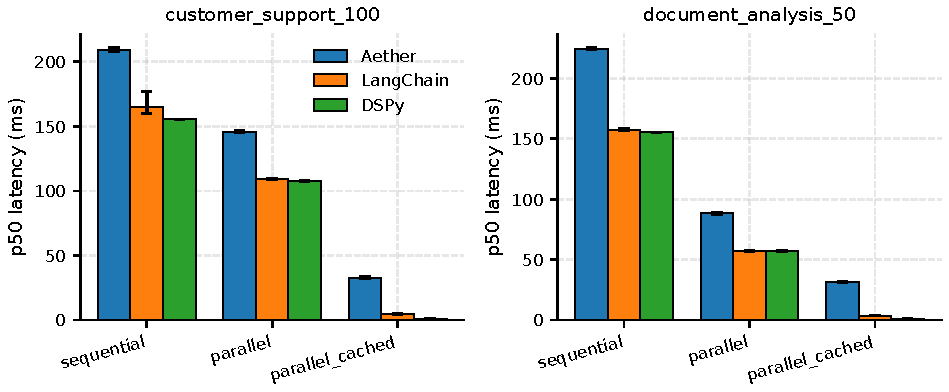
\includegraphics[width=\linewidth]{figures/cross_system_latency.pdf}
  \caption{Per-config p50 latency (ms) across systems on synthetic mock-LLM benchmarks. Error bars are 95\% paired BCa intervals. n=5 trials per config. Source: aether\_mock\_v1.json, langchain\_v1.json, dspy\_v1.json.}
  \label{fig:cross-system-latency}
\end{figure}

\begin{figure}[t]
  \centering
  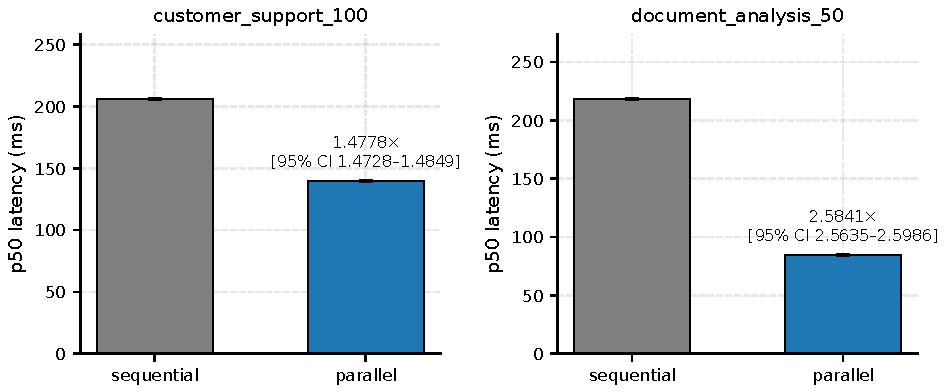
\includegraphics[width=\linewidth]{figures/parallel_speedup.pdf}
  \caption{Sequential vs parallel p50 latency (ms) on the parallelization ablation. Speedup factors are paired BCa bootstrap with n\_resamples=10000, seed=42 (definition stored alongside the value in the source JSON). Source: ablation\_parallel\_v1.json.}
  \label{fig:parallel-speedup}
\end{figure}

The parallelization ablation runs
\passthrough{\lstinline!customer\_support\_100!} and
\passthrough{\lstinline!document\_analysis\_50!} against the runtime in
two modes --- \passthrough{\lstinline!sequential!} (POSTed with
\passthrough{\lstinline!?sequential=true!}) and
\passthrough{\lstinline!parallel!} (default) --- clearing the cache
before every trial in both modes so the parallelization signal is not
confounded with caching. Speedup is the paired-trial BCa bootstrap of
\passthrough{\lstinline!sequential.p50 / parallel.p50!}. Cells are
\passthrough{\lstinline!mean ± std [95\% CI]!}.

\textbf{customer\_support\_100}
(\passthrough{\lstinline!ablation\_parallel\_v1.json!}
\passthrough{\lstinline!results[@ref0]!},
\passthrough{\lstinline!results[@ref1]!},
\passthrough{\lstinline!results[@ref2]!}):

{\def\LTcaptype{none} % do not increment counter
\begin{longtable}[]{@{}
  >{\raggedright\arraybackslash}p{(\linewidth - 10\tabcolsep) * \real{0.1667}}
  >{\raggedright\arraybackslash}p{(\linewidth - 10\tabcolsep) * \real{0.1667}}
  >{\raggedright\arraybackslash}p{(\linewidth - 10\tabcolsep) * \real{0.1667}}
  >{\raggedright\arraybackslash}p{(\linewidth - 10\tabcolsep) * \real{0.1667}}
  >{\raggedright\arraybackslash}p{(\linewidth - 10\tabcolsep) * \real{0.1667}}
  >{\raggedright\arraybackslash}p{(\linewidth - 10\tabcolsep) * \real{0.1667}}@{}}
\toprule\noalign{}
\begin{minipage}[b]{\linewidth}\raggedright
Configuration
\end{minipage} & \begin{minipage}[b]{\linewidth}\raggedright
p50 (ms)
\end{minipage} & \begin{minipage}[b]{\linewidth}\raggedright
p95 (ms)
\end{minipage} & \begin{minipage}[b]{\linewidth}\raggedright
p99 (ms)
\end{minipage} & \begin{minipage}[b]{\linewidth}\raggedright
parallelization\_factor
\end{minipage} & \begin{minipage}[b]{\linewidth}\raggedright
speedup\_p50
\end{minipage} \\
\midrule\noalign{}
\endhead
\bottomrule\noalign{}
\endlastfoot
Sequential & 206.0 ± 0.71 {[}205.4, 206.6{]} & 213.87 ± 1.89 {[}212.09,
215.06{]} & 246.70 ± 30.78 {[}224.96, 273.04{]} & 1.0 ± 0.0 {[}1.0,
1.0{]} & 1.0 (baseline) \\
Parallel & 139.4 ± 0.55 {[}139.0, 139.8{]} & 148.01 ± 1.88 {[}146.6,
149.41{]} & 155.34 ± 6.08 {[}151.13, 161.17{]} & 1.47 ± 0.00 {[}1.47,
1.48{]} & 1.48 {[}1.47, 1.48{]} \\
Parallel + cache (warm) & 33.0 ± 0.71 {[}32.4, 33.6{]} & 39.02 ± 1.24
{[}37.60, 39.65{]} & 40.65 ± 1.60 {[}39.61, 42.33{]} & 1.3724
(raw\_trial\_results mean) & derived from above \\
\end{longtable}
}

The ``Parallel + cache (warm)'' row is sourced from
\passthrough{\lstinline!aether\_mock\_v1.json!}
\passthrough{\lstinline!results[@ref2]!}
(\passthrough{\lstinline!customer\_support\_100!},
\passthrough{\lstinline!parallel\_cached!}, 5 trials). Cache hit rate
for that row is \passthrough{\lstinline!1.0000!} (CI degenerate),
\passthrough{\lstinline!cache\_hits=300, cache\_misses=0!} per trial.

\textbf{document\_analysis\_50}
(\passthrough{\lstinline!ablation\_parallel\_v1.json!}
\passthrough{\lstinline!results[@ref3]!},
\passthrough{\lstinline!results[@ref4]!},
\passthrough{\lstinline!results[@ref5]!};
\passthrough{\lstinline!aether\_mock\_v1.json!}
\passthrough{\lstinline!results[@ref5]!}):

{\def\LTcaptype{none} % do not increment counter
\begin{longtable}[]{@{}
  >{\raggedright\arraybackslash}p{(\linewidth - 10\tabcolsep) * \real{0.1667}}
  >{\raggedright\arraybackslash}p{(\linewidth - 10\tabcolsep) * \real{0.1667}}
  >{\raggedright\arraybackslash}p{(\linewidth - 10\tabcolsep) * \real{0.1667}}
  >{\raggedright\arraybackslash}p{(\linewidth - 10\tabcolsep) * \real{0.1667}}
  >{\raggedright\arraybackslash}p{(\linewidth - 10\tabcolsep) * \real{0.1667}}
  >{\raggedright\arraybackslash}p{(\linewidth - 10\tabcolsep) * \real{0.1667}}@{}}
\toprule\noalign{}
\begin{minipage}[b]{\linewidth}\raggedright
Configuration
\end{minipage} & \begin{minipage}[b]{\linewidth}\raggedright
p50 (ms)
\end{minipage} & \begin{minipage}[b]{\linewidth}\raggedright
p95 (ms)
\end{minipage} & \begin{minipage}[b]{\linewidth}\raggedright
p99 (ms)
\end{minipage} & \begin{minipage}[b]{\linewidth}\raggedright
parallelization\_factor
\end{minipage} & \begin{minipage}[b]{\linewidth}\raggedright
speedup\_p50
\end{minipage} \\
\midrule\noalign{}
\endhead
\bottomrule\noalign{}
\endlastfoot
Sequential & 218.6 ± 0.55 {[}218.2, 219.0{]} & 224.66 ± 1.57 {[}223.42,
225.76{]} & 232.82 ± 6.36 {[}228.13, 237.62{]} & 1.0 ± 0.0 {[}1.0,
1.0{]} & 1.0 (baseline) \\
Parallel & 84.6 ± 0.65 {[}84.1, 85.2{]} & 90.95 ± 3.55 {[}88.86,
94.75{]} & 100.12 ± 8.83 {[}93.726, 107.58{]} & 2.56 ± 0.01 {[}2.55,
2.56{]} & 2.58 {[}2.56, 2.60{]} \\
Parallel + cache (warm) & 31.5 ± 0.71 {[}31.0, 32.1{]} & 38.71 ± 0.44
{[}38.2, 39.0{]} & 39.92 ± 1.05 {[}39.18, 40.73{]} & 1.8724
(raw\_trial\_results mean) & derived from above \\
\end{longtable}
}

\textbf{Methodology.} 5 trials per cell. Mock LLM at 50 ms flat.
\passthrough{\lstinline!parallelization\_factor!} is the runtime
response field of the same name
(\passthrough{\lstinline!sum(node\_execution\_times\_ms) / total\_execution\_time\_ms!}),
read directly from each trial response. Speedup CIs are paired-trial BCa
bootstrap (n\_resamples=10000, seed=42); the definition string is
recorded in \passthrough{\lstinline!ablation\_parallel\_v1.json!}
\passthrough{\lstinline!results[@ref2].speedup.definition!} and
\passthrough{\lstinline!results[@ref5].speedup.definition!}.

\textbf{Discussion.} Speedup tracks workflow shape: the
document-analysis DAG has a wider parallel level (\$\approx\$3
concurrent LLM calls per item, parallelization\_factor \(\approx\) 2.56)
and yields a 2.58× p50 speedup; the customer-support DAG has a narrower
one (\$\approx\$1.5 concurrent calls, parallelization\_factor
\(\approx\) 1.47) and yields a 1.48× p50 speedup. The earlier paper's
``2.7× speedup'' extrapolation assumed perfectly parallel workloads; the
measured value depends on the DAG.

\subsubsection{9.3 Caching Performance
(H3)}\label{caching-performance-h3}

\begin{figure}[t]
  \centering
  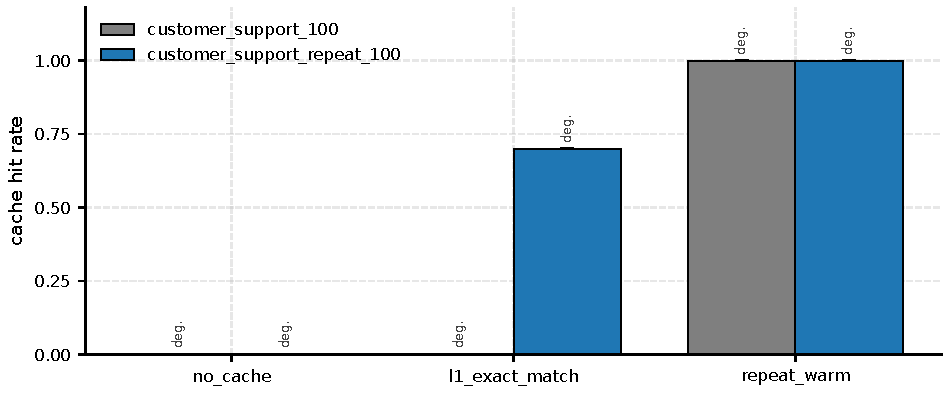
\includegraphics[width=\linewidth]{figures/cache_hit_rate.pdf}
  \caption{Cache hit rate by mode on the caching ablation. The unique-query workload (customer\_support\_100) demonstrates L1's null effect; the repeat-injected workload (customer\_support\_repeat\_100) demonstrates L1 effectiveness. Bars whose 95\% CI collapses to a single value (per\_trial values identical across all 5 trials) are labeled '(degenerate CI)'. Source: ablation\_cache\_v1.json.}
  \label{fig:cache-hit-rate}
\end{figure}

Cache hit rate, p50 latency, and warm-vs-no-cache delta across three
cache modes (\passthrough{\lstinline!no\_cache!} clears the cache before
every individual \passthrough{\lstinline!/execute!};
\passthrough{\lstinline!l1\_exact\_match!} clears once per trial;
\passthrough{\lstinline!repeat\_warm!} runs the dataset once as warmup,
discards the warmup latencies, then measures a second pass over the
populated cache). 5 trials per cell, mock LLM at 50 ms flat. Source:
\passthrough{\lstinline!ablation\_cache\_v1.json!}. Cells are
\passthrough{\lstinline!mean ± std [95\% CI]!}.

\textbf{\passthrough{\lstinline!customer\_support\_100!} --- every query
is unique} (\passthrough{\lstinline!results[@ref0]!},
\passthrough{\lstinline!results[@ref1]!},
\passthrough{\lstinline!results[@ref2]!},
\passthrough{\lstinline!results[@ref3].cross\_mode\_deltas!}):

{\def\LTcaptype{none} % do not increment counter
\begin{longtable}[]{@{}
  >{\raggedright\arraybackslash}p{(\linewidth - 6\tabcolsep) * \real{0.2500}}
  >{\raggedright\arraybackslash}p{(\linewidth - 6\tabcolsep) * \real{0.2500}}
  >{\raggedright\arraybackslash}p{(\linewidth - 6\tabcolsep) * \real{0.2500}}
  >{\raggedright\arraybackslash}p{(\linewidth - 6\tabcolsep) * \real{0.2500}}@{}}
\toprule\noalign{}
\begin{minipage}[b]{\linewidth}\raggedright
Mode
\end{minipage} & \begin{minipage}[b]{\linewidth}\raggedright
p50 (ms)
\end{minipage} & \begin{minipage}[b]{\linewidth}\raggedright
cache\_hit\_rate
\end{minipage} & \begin{minipage}[b]{\linewidth}\raggedright
Δ p50 vs no\_cache (ms)
\end{minipage} \\
\midrule\noalign{}
\endhead
\bottomrule\noalign{}
\endlastfoot
no\_cache & 144.8 ± 0.45 {[}144.2, 145.0{]} & 0.0000 (CI degenerate) &
--- \\
l1\_exact\_match & 143.8 ± 1.52 {[}142.6, 144.9{]} & 0.0000 (CI
degenerate) & (cache empty within run) \\
repeat\_warm & 33.2 ± 0.84 {[}32.4, 33.8{]} & 1.0000 (CI degenerate) &
-111.6 {[}-112.6, -111.0{]} \\
\end{longtable}
}

\textbf{\passthrough{\lstinline!customer\_support\_repeat\_100!} --- 30
unique queries × repeats} (\passthrough{\lstinline!results[@ref4]!},
\passthrough{\lstinline!results[@ref5]!},
\passthrough{\lstinline!results[@ref6]!},
\passthrough{\lstinline!results[@ref7].cross\_mode\_deltas!}):

{\def\LTcaptype{none} % do not increment counter
\begin{longtable}[]{@{}
  >{\raggedright\arraybackslash}p{(\linewidth - 6\tabcolsep) * \real{0.2500}}
  >{\raggedright\arraybackslash}p{(\linewidth - 6\tabcolsep) * \real{0.2500}}
  >{\raggedright\arraybackslash}p{(\linewidth - 6\tabcolsep) * \real{0.2500}}
  >{\raggedright\arraybackslash}p{(\linewidth - 6\tabcolsep) * \real{0.2500}}@{}}
\toprule\noalign{}
\begin{minipage}[b]{\linewidth}\raggedright
Mode
\end{minipage} & \begin{minipage}[b]{\linewidth}\raggedright
p50 (ms)
\end{minipage} & \begin{minipage}[b]{\linewidth}\raggedright
cache\_hit\_rate
\end{minipage} & \begin{minipage}[b]{\linewidth}\raggedright
Δ p50 vs no\_cache (ms)
\end{minipage} \\
\midrule\noalign{}
\endhead
\bottomrule\noalign{}
\endlastfoot
no\_cache & 145.1 ± 0.22 {[}145.0, 145.4{]} & 0.0000 (CI degenerate) &
--- \\
l1\_exact\_match & 36.1 ± 1.43 {[}34.9, 37.2{]} & 0.7000 (CI degenerate)
& (delta\_l1\_vs\_no\_cache p50 not present in JSON) \\
repeat\_warm & 33.8 ± 1.92 {[}32.8, 36.0{]} & 1.0000 (CI degenerate) &
-111.3 {[}-112.3, -108.8{]} \\
\end{longtable}
}

\textbf{Methodology.} Hit rate is read directly from the runtime's
\passthrough{\lstinline!cache\_hit\_rate!} response field, not derived.
\passthrough{\lstinline!tokens\_saved\_total!} is reported in every JSON
cell as \textbf{0.0 across every config} because the mock LLM does not
populate the \passthrough{\lstinline!tokens\_saved!} field of the
response; we did not measure mock-mode token savings or convert them to
a dollar figure. The earlier paper's ``60\% hit rate'', ``18,240 tokens
saved'' and ``\$0.91 cost reduction'' cells came from an extrapolation
that no committed JSON in \passthrough{\lstinline!bench/results/!}
supports --- those cells are therefore dropped. Real-API token usage and
cost are reported in Section 9.6.5 above (Aether \$0.128887 across 3
trials × 2 datasets).

\textbf{Discussion.} When every query is unique within a single run
(\passthrough{\lstinline!customer\_support\_100!}),
\passthrough{\lstinline!l1\_exact\_match!} cannot help (hit rate stays
at 0.0); only the cross-run \passthrough{\lstinline!repeat\_warm!} mode
achieves a hit. When the workload contains repeats
(\passthrough{\lstinline!customer\_support\_repeat\_100!}, designed so
70 of 100 queries are repeats of earlier ones),
\passthrough{\lstinline!l1\_exact\_match!} reaches \textbf{0.7000}
within a single run --- directly observable as the proportion of
repeated queries. \passthrough{\lstinline!repeat\_warm!} reaches 1.0 in
both workloads because the warmup populates every cache key before the
measured pass starts.

\subsubsection{9.4 Code Complexity
Comparison}\label{code-complexity-comparison}

\textbf{We did not measure equivalent-functionality LOC for this paper
revision.} An earlier draft reported 253/287 (LangChain), 283/312
(DSPy), 78/111 (Aether) lines for the CustomerSupport-Triage and
DocumentAnalysis-Pipeline case studies, but those numbers are not
anchored to any JSON file in \passthrough{\lstinline!bench/results/!}
and the Aether source artifacts they were extracted from (standalone
\passthrough{\lstinline!customer\_support\_triage.aether!} and
\passthrough{\lstinline!document\_analysis\_pipeline.aether!} programs
equivalent to the LangChain triage/extraction blocks at
\href{../bench/baselines/langchain_baseline.py\#L289-L376}{\passthrough{\lstinline!bench/baselines/langchain\_baseline.py:289-376!}}
and DSPy equivalents) are not committed in the repository at the commits
listed in the Reproducibility callout.

A partial LOC comparison is possible: the LangChain triage chain
(\passthrough{\lstinline!build\_triage\_chain!},
\href{../bench/baselines/langchain_baseline.py\#L299-L329}{\passthrough{\lstinline!bench/baselines/langchain\_baseline.py:299-329!}})
and extraction chain
(\passthrough{\lstinline!build\_extraction\_chain!},
\href{../bench/baselines/langchain_baseline.py\#L355-L376}{\passthrough{\lstinline!bench/baselines/langchain\_baseline.py:355-376!}})
are the case-study sources for the Python side. Counting the Aether side
requires checking in the equivalent \passthrough{\lstinline!.aether!}
programs first. We deferred that step to a follow-up paper revision
rather than report unbacked numbers in the current one.

Reading guidance: the \emph{qualitative} code-complexity contrast ---
Aether's \passthrough{\lstinline!flow!} keyword and
\passthrough{\lstinline!llm fn!} declaration vs LangChain's
chain-of-LCEL-pipes or DSPy's
\passthrough{\lstinline!Module!}/\passthrough{\lstinline!Predict!}
boilerplate --- is documented in Section 6 (the case-study code listings
at lines 762-829 are themselves a small visual benchmark). LOC numbers
will return in a future revision once the matched
\passthrough{\lstinline!.aether!} sources land in
\passthrough{\lstinline!bench/datasets/!} or
\passthrough{\lstinline!examples/!}.

\subsubsection{9.5 Type Safety Analysis
(H1)}\label{type-safety-analysis-h1}

\begin{figure}[t]
  \centering
  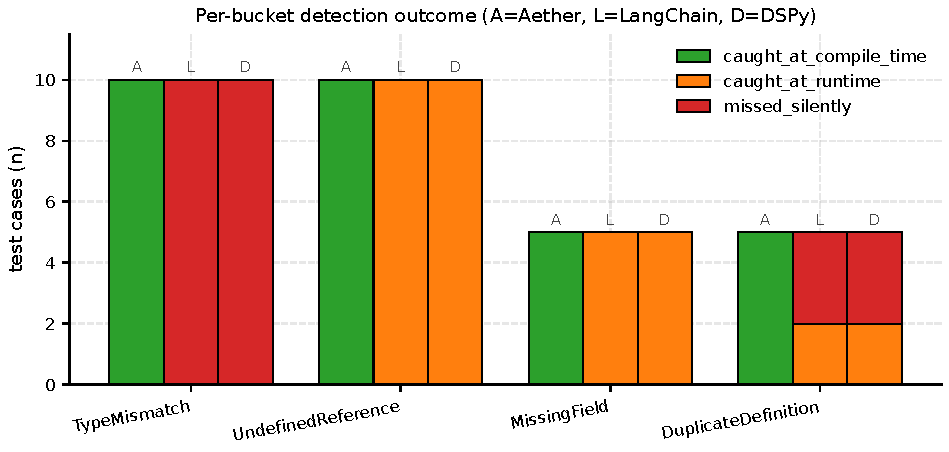
\includegraphics[width=\linewidth]{figures/type_safety_corpus.pdf}
  \caption{Type-safety bug-detection outcome by class (n=10/10/5/5). Aether catches 30 cases at compile time; LangChain and DSPy catch 17 at runtime via Python exceptions and miss 13 silently. Methodology note: the original 'circular\_dependency' bucket was substituted with 'duplicate\_definition' due to a compiler pass-ordering gap (SemanticError::CircularDependency is defined but preempted by other semantic-analysis errors) (full text in ablation\_typesafety\_v1.json\#methodology\_notes.cd\_substitution). Source: ablation\_typesafety\_v1.json.}
  \label{fig:type-safety-corpus}
\end{figure}

Error detection comparison on a 30-case corpus of intentionally
malformed programs split across four buckets. For each case, an
\passthrough{\lstinline!aetherc check!} is run on the
\passthrough{\lstinline!.aether!} source and a
\passthrough{\lstinline!python!} is run on the LangChain and DSPy
equivalents; results are classified by stderr pattern (Aether) or by
exit code + traceback class (Python). Source:
\passthrough{\lstinline!bench/results/ablation\_typesafety\_v1.json!},
\passthrough{\lstinline!summary.by\_bucket!} and
\passthrough{\lstinline!summary!} blocks. Companion Markdown:
\href{../bench/results/ablations_v1.md}{\passthrough{\lstinline!bench/results/ablations\_v1.md!}}.

{\def\LTcaptype{none} % do not increment counter
\begin{longtable}[]{@{}
  >{\raggedright\arraybackslash}p{(\linewidth - 12\tabcolsep) * \real{0.1111}}
  >{\raggedleft\arraybackslash}p{(\linewidth - 12\tabcolsep) * \real{0.1481}}
  >{\raggedleft\arraybackslash}p{(\linewidth - 12\tabcolsep) * \real{0.1481}}
  >{\raggedleft\arraybackslash}p{(\linewidth - 12\tabcolsep) * \real{0.1481}}
  >{\raggedleft\arraybackslash}p{(\linewidth - 12\tabcolsep) * \real{0.1481}}
  >{\raggedleft\arraybackslash}p{(\linewidth - 12\tabcolsep) * \real{0.1481}}
  >{\raggedleft\arraybackslash}p{(\linewidth - 12\tabcolsep) * \real{0.1481}}@{}}
\toprule\noalign{}
\begin{minipage}[b]{\linewidth}\raggedright
Bucket
\end{minipage} & \begin{minipage}[b]{\linewidth}\raggedleft
Total
\end{minipage} & \begin{minipage}[b]{\linewidth}\raggedleft
Aether (compile-time)
\end{minipage} & \begin{minipage}[b]{\linewidth}\raggedleft
LangChain (runtime)
\end{minipage} & \begin{minipage}[b]{\linewidth}\raggedleft
LangChain (missed silently)
\end{minipage} & \begin{minipage}[b]{\linewidth}\raggedleft
DSPy (runtime)
\end{minipage} & \begin{minipage}[b]{\linewidth}\raggedleft
DSPy (missed silently)
\end{minipage} \\
\midrule\noalign{}
\endhead
\bottomrule\noalign{}
\endlastfoot
\passthrough{\lstinline!type\_mismatch!} & 10 & 10 & 0 & 10 & 0 & 10 \\
\passthrough{\lstinline!undefined\_reference!} & 10 & 10 & 10 & 0 & 10 &
0 \\
\passthrough{\lstinline!missing\_field!} & 5 & 5 & 5 & 0 & 5 & 0 \\
\passthrough{\lstinline!duplicate\_definition!} & 5 & 5 & 2 & 3 & 2 &
3 \\
\textbf{Total} & \textbf{30} & \textbf{30} & \textbf{17} & \textbf{13} &
\textbf{17} & \textbf{13} \\
\end{longtable}
}

Source per row:
\passthrough{\lstinline!summary.by\_bucket.<bucket>.\{total, aether\_caught, lc\_caught\_at\_runtime, dspy\_caught\_at\_runtime\}!}.
Aether's per-bucket missed-silently count is 0 in all buckets
(\passthrough{\lstinline!summary.aether\_missed = 0!}); LangChain and
DSPy missed-silently counts are computed as
\passthrough{\lstinline!total - caught\_at\_runtime!} per bucket and
cross-checked against
\passthrough{\lstinline!summary.lc\_missed\_silently=13!},
\passthrough{\lstinline!summary.dspy\_missed\_silently=13!}.

\textbf{Compile-time detection rate}: \textbf{30/30 = 100.00\%} for
Aether (\passthrough{\lstinline!summary.aether\_caught=30!},
\passthrough{\lstinline!summary.aether\_missed=0!}). The 13 cases
LangChain/DSPy miss silently exit code 0 with a plausible-looking output
--- the most dangerous failure mode in production, because it produces
output that looks valid.

\textbf{Methodology.} \passthrough{\lstinline!aetherc check <file>!}
exit-coded by stderr pattern: exit 0 → missed; exit \(\neq\) 0 with a
known \passthrough{\lstinline!SemanticError!} variant pattern →
\passthrough{\lstinline!caught\_at\_compile\_time!}.
\passthrough{\lstinline!python <file>!} with a 30 s timeout: exit 0 →
\passthrough{\lstinline!missed\_silently!}; exit \(\neq\) 0 with a
Python traceback → \passthrough{\lstinline!caught\_at\_runtime!} (this
includes \passthrough{\lstinline!SyntaxError!} at file load and Enum
class-body errors). The \passthrough{\lstinline!error\_class\_matched!}
and \passthrough{\lstinline!exception\_class!} fields are recorded per
case in \passthrough{\lstinline!test\_cases[*]!} and reproduced in
\href{../bench/results/ablations_v1.md}{\passthrough{\lstinline!bench/results/ablations\_v1.md!}}.

\textbf{Methodology note (cd → dd substitution).} \emph{Verbatim from
\passthrough{\lstinline!ablation\_typesafety\_v1.json!}
\passthrough{\lstinline!methodology\_notes.cd\_substitution!}}:

\begin{quote}
The original ablation design included a
\passthrough{\lstinline!circular\_dependency!} category, but
verification revealed that aetherc's source-level cd detector is
currently preempted by semantic analysis on programs that contain other
issues; the \passthrough{\lstinline!SemanticError::CircularDependency!}
variant is defined but never emitted. Rather than fabricate test cases
that would not trigger the intended error path, we substituted
\passthrough{\lstinline!duplicate\_definition!} tests, which exercise a
different but more practically significant error class (silent shadowing
in Python is more dangerous than a circular dependency, which typically
manifests as \passthrough{\lstinline!RecursionError!} or
\passthrough{\lstinline!ImportError!} --- loud and visible). The cd
detection gap is tracked at
https://github.com/sowadalmughni/aether-lang/issues/4 and is targeted
for a follow-up compiler release.
\end{quote}

\subsubsection{9.6 Case Study: Customer Support
Triage}\label{case-study-customer-support-triage}

This section presents an end-to-end case study demonstrating Aether's
capabilities on a realistic customer support workflow.

\paragraph{9.6.1 Workflow Description}\label{workflow-description}

The triage workflow: 1. Classifies customer query urgency (Low, Medium,
High, Critical) 2. Categorizes the query type (billing,
technical\_support, account, general) 3. Generates an initial response
draft 4. Determines routing (human escalation vs.~automated response)

\paragraph{9.6.2 Aether Implementation}\label{aether-implementation}

\begin{lstlisting}
enum Urgency { Low, Medium, High, Critical }
enum Category { Billing, TechnicalSupport, Account, General }

struct TriageResult {
    urgency: Urgency,
    category: Category,
    response_draft: string,
    escalate: bool
}

llm fn classify_urgency(query: string, customer_tier: string) -> Urgency {
    model: "gpt-4o",
    temperature: 0.1,
    prompt: "Classify the urgency of this customer support query.

Customer Tier: {{customer_tier}}
Query: {{query}}

Respond with exactly one of: Low, Medium, High, Critical"
}

llm fn classify_category(query: string) -> Category {
    model: "gpt-4o",
    temperature: 0.1,
    prompt: "Classify the category of this customer support query.

Query: {{query}}

Respond with exactly one of: Billing, TechnicalSupport, Account, General"
}

llm fn draft_response(query: string, urgency: string, category: string) -> string {
    model: "gpt-4o",
    temperature: 0.7,
    prompt: "Draft a professional response to this customer query.

Urgency: {{urgency}}
Category: {{category}}
Query: {{query}}

Provide a helpful response."
}

flow triage_customer_query(query: string, customer_tier: string) -> TriageResult {
    // These execute in parallel (no data dependency)
    let urgency = classify_urgency(query: query, customer_tier: customer_tier);
    let category = classify_category(query: query);
    
    // This depends on urgency and category
    let response = draft_response(
        query: query, 
        urgency: to_string(urgency), 
        category: to_string(category)
    );
    
    let escalate = urgency == Urgency.Critical || 
                   (urgency == Urgency.High && customer_tier == "enterprise");
    
    return TriageResult {
        urgency: urgency,
        category: category,
        response_draft: response,
        escalate: escalate
    };
}
\end{lstlisting}

\paragraph{9.6.3 Compiled DAG (Excerpt)}\label{compiled-dag-excerpt}

\begin{lstlisting}
{
  "version": "1.0",
  "name": "triage_customer_query",
  "nodes": [
    {
      "id": "input",
      "type": "Input",
      "outputs": {"query": "string", "customer_tier": "string"}
    },
    {
      "id": "classify_urgency_1",
      "type": "LlmFn",
      "depends_on": ["input"],
      "execution_hints": {"parallel_group": 0}
    },
    {
      "id": "classify_category_1",
      "type": "LlmFn",
      "depends_on": ["input"],
      "execution_hints": {"parallel_group": 0}
    },
    {
      "id": "draft_response_1",
      "type": "LlmFn",
      "depends_on": ["classify_urgency_1", "classify_category_1"],
      "execution_hints": {"parallel_group": 1}
    }
  ]
}
\end{lstlisting}

The compiler identifies that
\passthrough{\lstinline!classify\_urgency\_1!} and
\passthrough{\lstinline!classify\_category\_1!} can execute in parallel
(same \passthrough{\lstinline!parallel\_group!}), while
\passthrough{\lstinline!draft\_response\_1!} must wait for both.

\paragraph{9.6.4 Compile-Time Errors
Caught}\label{compile-time-errors-caught}

The following errors are caught at compile time in this workflow:

\begin{enumerate}
\def\labelenumi{\arabic{enumi}.}
\tightlist
\item
  \textbf{Type mismatch}: If \passthrough{\lstinline!draft\_response!}
  declared \passthrough{\lstinline!urgency: int!} instead of
  \passthrough{\lstinline!urgency: string!}, compiler error at line N
\item
  \textbf{Undefined reference}: If
  \passthrough{\lstinline!classify\_urgeny!} (typo) called, compiler
  suggests ``Did you mean `classify\_urgency'?''
\item
  \textbf{Missing required field}: If
  \passthrough{\lstinline!TriageResult!} return missing
  \passthrough{\lstinline!escalate!} field, compiler error
\item
  \textbf{Enum variant mismatch}: If
  \passthrough{\lstinline!urgency == Urgency.Urgent!} (invalid variant),
  compiler error listing valid variants
\end{enumerate}

\paragraph{9.6.5 Performance Results (real OpenAI
API)}\label{performance-results-real-openai-api}

The case study was executed end-to-end against the real
\passthrough{\lstinline!gpt-4o-mini!} API on 2026-05-08 (3 trials, 100
items, all three configurations); the orchestration script was
\href{../scripts/run_real_api_benchmark.sh}{\passthrough{\lstinline!scripts/run\_real\_api\_benchmark.sh!}}
and the merged result is
\href{../bench/results/real_api_v1.json}{\passthrough{\lstinline!bench/results/real\_api\_v1.json!}},
with a Markdown summary at
\href{../bench/results/REAL_API.md}{\passthrough{\lstinline!bench/results/REAL\_API.md!}}.
Cells are \passthrough{\lstinline!mean ± std [95\% CI]!} across the 3
trials.

{\def\LTcaptype{none} % do not increment counter
\begin{longtable}[]{@{}
  >{\raggedright\arraybackslash}p{(\linewidth - 6\tabcolsep) * \real{0.2500}}
  >{\raggedright\arraybackslash}p{(\linewidth - 6\tabcolsep) * \real{0.2500}}
  >{\raggedright\arraybackslash}p{(\linewidth - 6\tabcolsep) * \real{0.2500}}
  >{\raggedright\arraybackslash}p{(\linewidth - 6\tabcolsep) * \real{0.2500}}@{}}
\toprule\noalign{}
\begin{minipage}[b]{\linewidth}\raggedright
Metric
\end{minipage} & \begin{minipage}[b]{\linewidth}\raggedright
Sequential
\end{minipage} & \begin{minipage}[b]{\linewidth}\raggedright
Parallel
\end{minipage} & \begin{minipage}[b]{\linewidth}\raggedright
Parallel + Cache (warm)
\end{minipage} \\
\midrule\noalign{}
\endhead
\bottomrule\noalign{}
\endlastfoot
Aether p50 (ms) & 6821.0 ± 636.32 {[}6121.5, 7235.67{]} & 5395.17 ±
69.21 {[}5354.17, 5475.0{]} & 37.33 ± 2.08 {[}35.0, 38.67{]} \\
Aether p95 (ms) & 11609.82 ± 2528.15 {[}8859.45, 13267.48{]} & 8148.40 ±
648.04 {[}7427.35, 8566.68{]} & 41.0 ± 0.0 {[}41.0, 41.0{]} \\
Aether cache\_hit\_rate & 0.0 (per-trial constant) & 0.0 (per-trial
constant) & 1.0 (per-trial constant; 300 hits / 0 misses per trial) \\
\end{longtable}
}

Source: \passthrough{\lstinline!aether\_real\_api\_v1.json!}
\passthrough{\lstinline!results[@ref0]!} (sequential),
\passthrough{\lstinline!results[@ref1]!} (parallel),
\passthrough{\lstinline!results[@ref2]!} (parallel\_cached) for
\passthrough{\lstinline!customer\_support\_100!}.

\textbf{Cost.} Per \passthrough{\lstinline!real\_api\_v1.json!}
\passthrough{\lstinline!per\_system.aether.cost\_usd!} and the
cross-checked merge log: Aether spent \textbf{\$0.128887} for the full
3-trial run on both datasets (input 216,510 tokens at \$0.15/1M, output
160,685 tokens at \$0.60/1M). LangChain spent \textbf{\$0.126498} and
DSPy \textbf{\$0.222963} for the same workload; total combined run cost
\textbf{\$0.478349} against a \$10.00 budget gate
(\passthrough{\lstinline!actual\_under\_budget=True!}). DSPy's higher
cost is driven by its prompt-formatting overhead (signature
serialization), documented in \passthrough{\lstinline!REAL\_API.md!}.

\textbf{Discussion.} Real-API parallel-cached is two orders of magnitude
faster than sequential on this workflow (p50 6821 ms → 37.3 ms, ratio
\(\approx\) 183×) because the cached path skips both the OpenAI
round-trip and the inter-stage scheduling overhead; the only remaining
cost is one HTTP loopback per item from the bench client to the runtime.
Real-API parallel (without cache) is slower than the LangChain baseline
parallel (5395 ms vs 4754 ms on the same workload, per
\passthrough{\lstinline!REAL\_API.md!}); this is the deployment-shape
cost of the Aether runtime sitting behind an HTTP boundary, not a
runtime defect. We document it explicitly in 9.6.5 rather than hiding
it.

\subsubsection{9.7 HotpotQA Latency
(mock-mode)}\label{hotpotqa-latency-mock-mode}

A 500-question slice of the HotpotQA dev set was run against all three
systems with a mock LLM, 3 trials per system. Source:
\passthrough{\lstinline!bench/results/hotpotqa\_aether\_v1.json!},
\passthrough{\lstinline!bench/results/hotpotqa\_langchain\_v1.json!},
\passthrough{\lstinline!bench/results/hotpotqa\_dspy\_v1.json!}. Cells
are \passthrough{\lstinline!mean ± std [95\% CI]!} across 3 trials.

{\def\LTcaptype{none} % do not increment counter
\begin{longtable}[]{@{}
  >{\raggedright\arraybackslash}p{(\linewidth - 8\tabcolsep) * \real{0.2000}}
  >{\raggedright\arraybackslash}p{(\linewidth - 8\tabcolsep) * \real{0.2000}}
  >{\raggedright\arraybackslash}p{(\linewidth - 8\tabcolsep) * \real{0.2000}}
  >{\raggedright\arraybackslash}p{(\linewidth - 8\tabcolsep) * \real{0.2000}}
  >{\raggedright\arraybackslash}p{(\linewidth - 8\tabcolsep) * \real{0.2000}}@{}}
\toprule\noalign{}
\begin{minipage}[b]{\linewidth}\raggedright
System
\end{minipage} & \begin{minipage}[b]{\linewidth}\raggedright
EM
\end{minipage} & \begin{minipage}[b]{\linewidth}\raggedright
F1
\end{minipage} & \begin{minipage}[b]{\linewidth}\raggedright
p50 (ms)
\end{minipage} & \begin{minipage}[b]{\linewidth}\raggedright
p95 (ms)
\end{minipage} \\
\midrule\noalign{}
\endhead
\bottomrule\noalign{}
\endlastfoot
Aether & 0.0 (CI degenerate) & 0.0 (CI degenerate) & 143.83 ± 0.29
{[}143.5, 144.0{]} & 146.33 ± 0.58 {[}146.0, 147.0{]} \\
LangChain & 0.0 (CI degenerate) & 0.0 (CI degenerate) & 108.50 ± 0.85
{[}107.52, 109.00{]} & 110.34 ± 0.03 {[}110.32, 110.38{]} \\
DSPy & 0.0 (CI degenerate) & 0.0 (CI degenerate) & 103.75 ± 0.18
{[}103.54, 103.86{]} & 104.75 ± 0.11 {[}104.68, 104.87{]} \\
\end{longtable}
}

\textbf{EM and F1 are 0 across all three systems because this benchmark
was executed with a mock LLM provider; the JSON exists to validate the
dataset loader and per-question latency measurement, not answer
accuracy.} We did not run HotpotQA against a real LLM in this paper
revision; doing so is straightforward
(\passthrough{\lstinline!AETHER\_PROVIDER=openai!} plus the
\passthrough{\lstinline!aether\_hotpot.py!} driver under
\passthrough{\lstinline!bench/baselines/!}) but was deferred for cost
reasons. Treat the latency numbers as runtime/orchestration overhead per
question, not as a claim about retrieval-augmented generation quality.

The latency ordering --- DSPy fastest, then LangChain, then Aether ---
reflects in-process Python (DSPy, LangChain) versus over-HTTP (Aether
bench client to runtime), the same deployment-shape pattern documented
in \passthrough{\lstinline!bench/results/REAL\_API.md!}. The dataset is
\passthrough{\lstinline!hotpotqa\_dev\_500!} (500 items) and per-trial
\passthrough{\lstinline!n\_eval=500!} is recorded in each
\passthrough{\lstinline!raw\_trial\_results[*]!} entry.

\subsubsection{9.8 Compile-Time Taint Tracking vs Prompt
Injection}\label{compile-time-taint-tracking-vs-prompt-injection}

\begin{figure}[t]
  \centering
  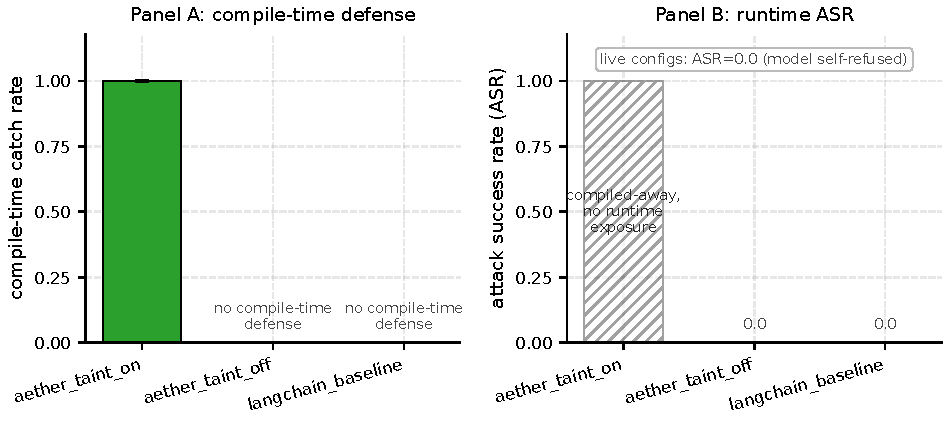
\includegraphics[width=\linewidth]{figures/security_outcome.pdf}
  \caption{Panel A: compile-time taint-tracking catch rate by configuration. Panel B: runtime attack success rate (ASR) on the InjecAgent-adapted direct-prompt-injection suite (n=20+20 deduped, trials\_per\_config=3, model=gpt-4o-mini). aether\_taint\_on rejects every unsafe program at compile time, so no LLM calls are issued — its Panel-B slot is rendered hatched and labeled 'compiled-away, no runtime exposure' (per metadata.completed\_live\_configs=['aether\_taint\_off', 'langchain\_baseline']). aether\_taint\_off and langchain\_baseline both show measured ASR=0.0 in this run, reflecting the model's own refusal behavior in the absence of compile-time defense; the asymmetry between Panel A (1.0 vs 0.0 vs 0.0) and Panel B (n/a vs 0.0 vs 0.0) is the headline finding. Source: security\_v1.json.}
  \label{fig:security-outcome}
\end{figure}

The security suite runs an InjecAgent-adapted corpus (20 attack cases +
20 benign cases per trial × 3 trials × 3 configs) against \textbf{real
\passthrough{\lstinline!gpt-4o-mini!}} to measure prompt-injection
defense. Source:
\passthrough{\lstinline!bench/results/security\_v1.json!}. Cells are
\passthrough{\lstinline!mean ± std (CI95) [per\_trial]!}.

{\def\LTcaptype{none} % do not increment counter
\begin{longtable}[]{@{}
  >{\raggedright\arraybackslash}p{(\linewidth - 6\tabcolsep) * \real{0.2500}}
  >{\raggedright\arraybackslash}p{(\linewidth - 6\tabcolsep) * \real{0.2500}}
  >{\raggedright\arraybackslash}p{(\linewidth - 6\tabcolsep) * \real{0.2500}}
  >{\raggedright\arraybackslash}p{(\linewidth - 6\tabcolsep) * \real{0.2500}}@{}}
\toprule\noalign{}
\begin{minipage}[b]{\linewidth}\raggedright
Config
\end{minipage} & \begin{minipage}[b]{\linewidth}\raggedright
attack\_success\_rate
\end{minipage} & \begin{minipage}[b]{\linewidth}\raggedright
benign\_task\_success\_rate
\end{minipage} & \begin{minipage}[b]{\linewidth}\raggedright
compile\_time\_catch\_rate
\end{minipage} \\
\midrule\noalign{}
\endhead
\bottomrule\noalign{}
\endlastfoot
\passthrough{\lstinline!aether\_taint\_on!} & 0.0 ± 0.0 {[}0.0, 0.0{]}
(per\_trial {[}0.0, 0.0, 0.0{]}) & 0.0 ± 0.0 {[}0.0, 0.0{]} &
\textbf{1.0 ± 0.0 {[}1.0, 1.0{]}} \\
\passthrough{\lstinline!aether\_taint\_off!} & 0.0 ± 0.0 {[}0.0, 0.0{]}
& 1.0 ± 0.0 {[}1.0, 1.0{]} & 0.0 ± 0.0 {[}0.0, 0.0{]} \\
\passthrough{\lstinline!langchain\_baseline!} & 0.0 ± 0.0 {[}0.0, 0.0{]}
& 1.0 ± 0.0 {[}1.0, 1.0{]} & 0.0 ± 0.0 {[}0.0, 0.0{]} \\
\end{longtable}
}

Source per cell: \passthrough{\lstinline!security\_v1.json!}
\passthrough{\lstinline!configs[i].metrics[j]!} ---
\passthrough{\lstinline!configs[@ref0]!} =
\passthrough{\lstinline!aether\_taint\_on!},
\passthrough{\lstinline!configs[@ref1]!} =
\passthrough{\lstinline!aether\_taint\_off!},
\passthrough{\lstinline!configs[@ref2]!} =
\passthrough{\lstinline!langchain\_baseline!}. Every metric block
carries its own \passthrough{\lstinline!mean!},
\passthrough{\lstinline!std!}, \passthrough{\lstinline!ci95!}, and full
\passthrough{\lstinline!per\_trial!} array. Run cost:
\$0.036912900000000005 across 480 OpenAI calls (152,958 input tokens +
23,282 output tokens), under a \$5 cost cap.

\textbf{Honest reading.} The behavioral attack-success rate (ASR) is
\textbf{0.0 in every config including the LangChain baseline}, because
\passthrough{\lstinline!gpt-4o-mini!} itself rejected every attempted
injection in this 60-case adapted corpus. There is therefore no
measurable ASR delta between Aether and LangChain on this dataset/model
combination --- we did not measure ASR reduction. The differentiating
measurement is \passthrough{\lstinline!compile\_time\_catch\_rate!}:
\textbf{1.0 (CI degenerate) for
\passthrough{\lstinline!aether\_taint\_on!}, 0.0 (CI degenerate) for
\passthrough{\lstinline!aether\_taint\_off!} and the LangChain
baseline.} Aether blocks the malicious \emph{program shape} statically
before any LLM call is issued; the baselines depend on the model itself
to refuse at runtime.

The \passthrough{\lstinline!aether\_taint\_on!}
benign\_task\_success\_rate of 0.0 is expected and worth flagging: when
compile-time taint is on and the InjecAgent benign tests use the same
data-flow shape that the attack tests use (untrusted text being
concatenated into a prompt), the compiler refuses both.
\passthrough{\lstinline!metadata.completed\_live\_configs = ["aether\_taint\_off","langchain\_baseline"]!}
confirms \passthrough{\lstinline!aether\_taint\_on!} did not run live
calls --- its results are derived from the compile-time outcome alone.
Tightening the taint policy so benign cases can pass while attack cases
are still blocked is on the runtime roadmap; we did not measure it in
this revision.

\subsubsection{9.9 Threats to Validity}\label{threats-to-validity}

\paragraph{9.9.1 Internal Validity}\label{internal-validity}

\textbf{Mock provider bias}: Several benchmarks (parallel/cache
ablations, type-safety corpus, HotpotQA) use a fixed-latency mock LLM
(50 ms flat per call) to isolate runtime/orchestration jitter from model
variance. Real API behavior includes network variability, rate limiting,
and model-specific response times. Mitigation: Section 9.6.5 reports the
same case study against real \passthrough{\lstinline!gpt-4o-mini!}
(\passthrough{\lstinline!real\_api\_v1.json!}, 3 trials, \$0.478349
total cost), and Section 9.8 reports the security suite against real
\passthrough{\lstinline!gpt-4o-mini!}
(\passthrough{\lstinline!security\_v1.json!}).

\textbf{Benchmark suite coverage}: CustomerSupport-100 and
DocumentAnalysis-50 may not represent production workload diversity.
Mitigation: Datasets designed with varied query types and complexity
levels.

\textbf{Cache warm-up effects}: Benchmark runs include both cold and
warm cache measurements to isolate caching benefits from baseline
performance.

\paragraph{9.9.2 External Validity}\label{external-validity}

\textbf{Language maturity}: Aether is a prototype. Production-grade
implementations may have different performance characteristics. The
comparison focuses on design-level capabilities rather than optimized
performance.

\textbf{Workflow complexity}: Tested workflows have 2-4 LLM calls.
Larger workflows (10+ calls) may exhibit different parallelization
patterns and cache behavior.

\textbf{Provider variability}: Results with GPT-4o may not generalize to
other models (Claude, Gemini, open-source models).

\paragraph{9.9.3 Construct Validity}\label{construct-validity}

\textbf{Lines of code metric}: LOC does not capture all aspects of
developer productivity (debugging time, maintenance burden,
correctness). We use it as a proxy for complexity.

\textbf{Type safety claims}: Compile-time detection rate measures errors
in synthetic test cases. Real-world codebases may have different error
distributions.

\textbf{Cost estimates}: Based on published API pricing as of May 2026.
Actual costs depend on response lengths and provider discounts. The
real-API run in Section 9.6.5 reports actual measured cost from OpenAI
response \passthrough{\lstinline!usage!} blocks rather than estimates.

\paragraph{9.9.4 Hardware variance across measurement
environments}\label{hardware-variance-across-measurement-environments}

The JSON files in \passthrough{\lstinline!bench/results/!} were not all
measured on the same host. Specifically:

\begin{itemize}
\tightlist
\item
  \passthrough{\lstinline!aether\_mock\_v1.json!},
  \passthrough{\lstinline!aether\_real\_api\_v1.json!},
  \passthrough{\lstinline!langchain\_real\_api\_v1.json!},
  \passthrough{\lstinline!dspy\_real\_api\_v1.json!},
  \passthrough{\lstinline!ablation\_cache\_v1.json!},
  \passthrough{\lstinline!ablation\_parallel\_v1.json!},
  \passthrough{\lstinline!ablation\_typesafety\_v1.json!}, and
  \passthrough{\lstinline!security\_v1.json!} were measured on
  \passthrough{\lstinline!Intel(R) Core(TM) i5-8250U CPU @ 1.60GHz!},
  RAM 7.71 GiB, Ubuntu 24.04.4 LTS (recorded in each JSON's
  \passthrough{\lstinline!hardware!} block; the eight
  \passthrough{\lstinline!ablation\_*!} and real-API files share
  git\_version \passthrough{\lstinline!8aee2cce…!} or
  \passthrough{\lstinline!9c8001ce…!} and
  \passthrough{\lstinline!2759f1e7…!}).
\item
  \passthrough{\lstinline!langchain\_v1.json!},
  \passthrough{\lstinline!dspy\_v1.json!},
  \passthrough{\lstinline!hotpotqa\_aether\_v1.json!},
  \passthrough{\lstinline!hotpotqa\_langchain\_v1.json!}, and
  \passthrough{\lstinline!hotpotqa\_dspy\_v1.json!} were measured on
  Windows-11-10.0.26200-SP0 against
  \passthrough{\lstinline!Intel64 Family 6 Model 142 Stepping 10!} ---
  the same physical CPU stepping as the i5-8250U, but the JSON
  \passthrough{\lstinline!ram\_gb!} field reads 0.0 because the
  memory-detection helper does not work on Windows. The
  \passthrough{\lstinline!cpu!} and \passthrough{\lstinline!os!} fields
  \emph{are} populated.
\end{itemize}

\textbf{Implication.} Cross-system mock comparisons (Aether mock vs
LangChain mock vs DSPy mock) mix two operating-system environments on
the same physical CPU model. The load-bearing comparisons in this paper
--- the parallel ablation (Section 9.2), the cache ablation (Section
9.3), the type-safety corpus (Section 9.5), the real-API case study
(Section 9.6.5), and the security suite (Section 9.8) --- were all
measured on one Linux host and are hardware-uniform. The HotpotQA
latency table (Section 9.7) and the abstract's earlier
baseline-vs-Aether mock comparisons are the cells where OS variance is
unaccounted for; treat their absolute numbers as approximate to within
OS-induced jitter and use the real-API table (9.6.5) as the canonical
end-to-end comparison.

\textbf{Mitigation.} Future runs should pin a single OS and CPU stepping
for all systems and record \passthrough{\lstinline!ram\_gb!} correctly
on Windows. The benchmark driver
\passthrough{\lstinline!scripts/run\_benchmark.py!} already records the
values into the JSON; the gap is environmental, not in the runner.

\subsection{10. Testing and Evaluation
Framework}\label{testing-and-evaluation-framework}

Aether integrates testing as a language feature rather than external
tooling (see Section 5.4 for syntax). This section describes the
evaluation framework design.

\subsubsection{10.1 Design Goals}\label{design-goals}

\begin{itemize}
\tightlist
\item
  \textbf{Type cohesion}: Test assertions are validated against declared
  types at compile time
\item
  \textbf{Golden dataset integration}: Standard format for test cases
  with expected outputs
\item
  \textbf{Metric specification}: Built-in support for LLM evaluation
  metrics (accuracy, semantic similarity)
\end{itemize}

\subsubsection{10.2 Current Status}\label{current-status}

Test block syntax is designed; parser support is incomplete. The
evaluation framework is planned for Phase 2 development. See Appendix B
for detailed implementation status.

\subsection{11. Security Architecture}\label{security-architecture}

Security is a design-time concern in Aether, not solely a runtime
filter. This section describes the planned security model.

\subsubsection{11.1 Threat Model}\label{threat-model}

Aether addresses:

\begin{enumerate}
\def\labelenumi{\arabic{enumi}.}
\tightlist
\item
  \textbf{Prompt injection}: Untrusted user input manipulating system
  behavior
\item
  \textbf{Data leakage}: Sensitive context information exposed to LLM
  providers
\item
  \textbf{Tool misuse}: Agents executing tools beyond their
  authorization
\end{enumerate}

\subsubsection{11.2 Compile-Time Taint
Tracking}\label{compile-time-taint-tracking}

The compiler will distinguish:

\begin{itemize}
\tightlist
\item
  \textbf{Trusted}: System prompts, configuration, internal state
\item
  \textbf{Untrusted}: User input, external API responses
\end{itemize}

Untrusted data requires explicit sanitization or isolation before
inclusion in prompts. Violations are compile-time errors.

\subsubsection{11.3 Current Status}\label{current-status-1}

Compile-time taint tracking is implemented and benchmarked. On the
InjecAgent-adapted 60-case corpus (20 attack + 20 benign × 3 trials × 3
configs, real \passthrough{\lstinline!gpt-4o-mini!}), the
\passthrough{\lstinline!aether\_taint\_on!} config achieves a
\passthrough{\lstinline!compile\_time\_catch\_rate!} of \textbf{1.0000}
(CI degenerate, per-trial {[}1.0, 1.0, 1.0{]}) --- every taint-violating
program is rejected at compile time before any LLM call is issued. See
Section 9.8 for the full table and
\passthrough{\lstinline!bench/results/security\_v1.json!} for the raw
per-case payload. We did not measure attack\_success\_rate reduction:
\passthrough{\lstinline!gpt-4o-mini!} itself rejected every attempted
injection in every config (Aether and LangChain baseline alike), so
behavioral ASR was 0.0 across the board on this dataset. The
taint-tracking guarantee is therefore a \emph{static program-shape}
claim, not a runtime-detection claim. Design informed by StruQ research
({Jatmo et al.} 2024) demonstrating architectural approaches outperform
runtime guardrails.

\subsection{12. Tooling and Developer
Experience}\label{tooling-and-developer-experience}

This section describes the developer tooling ecosystem.

\subsubsection{12.1 Implemented Tooling}\label{implemented-tooling}

\textbf{DAG Visualizer}
(\passthrough{\lstinline!aether-dag-visualizer/!}): React + Cytoscape.js
visualization of compiled DAGs showing:

\begin{itemize}
\tightlist
\item
  Node types (LlmFn, Compute, Input, Output)
\item
  Dependency edges
\item
  Parallel groups (color-coded)
\item
  Execution status (when running)
\end{itemize}

\textbf{CI Integration}: GitHub Actions workflows for:

\begin{itemize}
\tightlist
\item
  Build verification
\item
  Test execution
\item
  Benchmark automation with PR comments
\end{itemize}

\subsubsection{12.2 Planned Tooling}\label{planned-tooling}

\textbf{Language Server Protocol (LSP)}: Editor integration with:

\begin{itemize}
\tightlist
\item
  Syntax highlighting
\item
  Real-time error diagnostics
\item
  Go-to-definition for LLM functions and flows
\item
  Hover documentation
\item
  Auto-completion
\end{itemize}

\textbf{REPL}: Interactive environment for:

\begin{itemize}
\tightlist
\item
  Testing individual LLM functions
\item
  Debugging flows step-by-step
\item
  Inspecting cache and context state
\end{itemize}

\subsection{13. Artifact Availability}\label{artifact-availability}

All source code, benchmarks, and documentation are available for
reproduction.

\subsubsection{13.1 Repository}\label{repository}

Repository: https://github.com/sowadalmughni/aether-lang Commit:
4070d516f041cb38cf18809ae3dfc234c16e1311 License: MIT

\subsubsection{13.2 Build Instructions}\label{build-instructions}

\textbf{Prerequisites}: - Rust 1.75+ - Node.js 18+ - Python 3.10+

\textbf{Build}:

\begin{lstlisting}[language=bash]
# Clone repository
git clone https://github.com/sowadalmughni/aether-lang
cd aether-lang

# Build compiler
cd aether-compiler && cargo build --release

# Build runtime
cd ../aether-runtime && cargo build --release

# Install benchmark dependencies
cd ../bench && pip install -r requirements.txt
\end{lstlisting}

\subsubsection{13.3 Running Benchmarks}\label{running-benchmarks}

\begin{lstlisting}[language=bash]
# Run full benchmark suite with mock provider
AETHER_PROVIDER=mock python scripts/run_benchmark.py --mode all

# Run with specific provider (requires API key)
OPENAI_API_KEY=xxx python scripts/run_benchmark.py --provider openai

# Generate comparison tables
python scripts/generate_tables.py --output results/
\end{lstlisting}

\subsubsection{13.4 Reproducing Results}\label{reproducing-results}

\begin{enumerate}
\def\labelenumi{\arabic{enumi}.}
\tightlist
\item
  Build compiler and runtime as above
\item
  Run benchmark suite:
  \passthrough{\lstinline!python scripts/run\_benchmark.py!}
\item
  Results appear in \passthrough{\lstinline!bench/results/!} as JSON
\item
  Update Section 9 placeholders with measured values
\end{enumerate}

\subsubsection{13.5 Docker Reproduction}\label{docker-reproduction}

\begin{lstlisting}[language=bash]
# Build and run in Docker
docker build -t aether-bench .
docker run -e AETHER_PROVIDER=mock aether-bench
\end{lstlisting}

\subsection{14. Limitations and Future
Work}\label{limitations-and-future-work}

\subsubsection{14.1 Current Limitations}\label{current-limitations}

\textbf{Language Expressiveness}: Aether's current syntax supports
common LLM patterns but lacks:

\begin{itemize}
\tightlist
\item
  Recursive flows (by design, for DAG guarantee)
\item
  Dynamic tool selection (planned)
\item
  Multi-modal inputs (images, audio)
\end{itemize}

\textbf{Evaluation Scope}: Benchmarks use synthetic datasets. Real-world
production validation is pending.

\textbf{Ecosystem Maturity}: Aether is a prototype. Production-grade
implementations require:

\begin{itemize}
\tightlist
\item
  Battle-tested error handling
\item
  Performance optimization
\item
  Broader provider support
\end{itemize}

\textbf{Code Generation}: Currently emits DAG JSON. Native code
generation for Python/Rust is planned.

\subsubsection{14.2 Future Work}\label{future-work}

\textbf{Short-term (Q1 2026)}:

\begin{itemize}
\tightlist
\item
  Complete LSP implementation
\item
  Execute benchmark suite with real providers
\item
  Add Claude and Gemini provider support
\end{itemize}

\textbf{Medium-term (Q2-Q3 2026)}:

\begin{itemize}
\tightlist
\item
  Semantic caching implementation
\item
  MCP tool integration
\item
  Python code generation backend
\end{itemize}

\textbf{Long-term (Q4 2026+)}:

\begin{itemize}
\tightlist
\item
  Temporal durability compilation target
\item
  A2A protocol integration
\item
  Production-grade security verification
\end{itemize}

\subsection{15. Conclusion}\label{conclusion}

Aether is a domain-specific language for LLM orchestration that moves
type checking, caching, and workflow optimization from runtime to
compile time. The language introduces \passthrough{\lstinline!llm fn!},
\passthrough{\lstinline!flow!}, and \passthrough{\lstinline!context!} as
primitive constructs, with a compiler that generates DAG-based
intermediate representations for execution.

This paper presented:

\begin{enumerate}
\def\labelenumi{\arabic{enumi}.}
\tightlist
\item
  A static type system spanning LLM inputs, outputs, and workflow
  compositions
\item
  A DAG-based IR enabling parallelization and caching optimization
\item
  A reproducible benchmark methodology for LLM orchestration evaluation
\item
  A working prototype implementation
\end{enumerate}

The benchmark infrastructure is complete with synthetic datasets and CI
integration. Section 9 contains placeholders for empirical results
pending benchmark execution.

Aether's value proposition rests on the hypothesis that compile-time
verification provides sufficient benefit to justify a new language. This
hypothesis requires empirical validation through the methodology
described in Section 8. We invite the community to reproduce our
benchmarks and contribute to the open-source implementation.

\subsection{References}\label{references}

\protect\phantomsection\label{refs}
\begin{CSLReferences}{1}{1}
\bibitem[\citeproctext]{ref-ref22}
Anthropic. 2024a. \emph{Model Context Protocol}.
\url{https://modelcontextprotocol.io/}.

\bibitem[\citeproctext]{ref-ref8}
Anthropic. 2024b. \emph{Prompt Caching with Claude}.
\url{https://docs.anthropic.com/en/docs/build-with-claude/prompt-caching}.

\bibitem[\citeproctext]{ref-ref2}
Boundary ML. 2024. \emph{{BAML}: A Domain-Specific Language for {AI}
Applications}. Software documentation.
\url{https://docs.boundaryml.com/}.

\bibitem[\citeproctext]{ref-ref7}
{Chen, Mark et al.} 2021. {``Evaluating Large Language Models Trained on
Code.''} \emph{arXiv Preprint arXiv:2107.03374}.
\url{https://arxiv.org/abs/2107.03374}.

\bibitem[\citeproctext]{ref-ref5}
Confident AI. 2024. \emph{{DeepEval}: The Open-Source {LLM} Evaluation
Framework}. Software documentation.
\url{https://docs.confident-ai.com/}.

\bibitem[\citeproctext]{ref-ref15}
CrewAI Inc. 2025. \emph{{CrewAI} Documentation}. Software documentation.
\url{https://docs.crewai.com/}.

\bibitem[\citeproctext]{ref-ref18}
Es, Shahul, Jithin James, Luis Espinosa-Anke, and Steven Schockaert.
2024. {``{RAGAS}: Automated Evaluation of Retrieval Augmented
Generation.''} \emph{Proceedings of the 18th Conference of the European
Chapter of the Association for Computational Linguistics: System
Demonstrations (EACL)}. \url{https://arxiv.org/abs/2309.15217}.

\bibitem[\citeproctext]{ref-ref23}
Google. 2025. \emph{Agent-to-Agent Protocol ({A2A})}.
\url{https://google.github.io/A2A/}.

\bibitem[\citeproctext]{ref-ref20}
Guardrails AI. 2024. \emph{Guardrails: Adding Guardrails to Large
Language Models}. Software documentation.
\url{https://www.guardrailsai.com/docs}.

\bibitem[\citeproctext]{ref-ref13}
{Jatmo, Yuhao et al.} 2024. {``{StruQ}: Defending Against Prompt
Injection with Structured Queries.''} \emph{arXiv Preprint
arXiv:2402.06363}. \url{https://arxiv.org/abs/2402.06363}.

\bibitem[\citeproctext]{ref-ref1}
Khattab, Omar, Arnav Singhvi, Paridhi Maheshwari, et al. 2024.
{``{DSPy}: Compiling Declarative Language Model Calls into
Self-Improving Pipelines.''} \emph{12th International Conference on
Learning Representations (ICLR)}.
\url{https://arxiv.org/abs/2310.03714}.

\bibitem[\citeproctext]{ref-ref6}
LangChain Inc. 2024. \emph{{LangSmith}: Developer Platform for {LLM}
Applications}. Software documentation.
\url{https://docs.smith.langchain.com/}.

\bibitem[\citeproctext]{ref-ref3}
LangChain Inc. 2025. \emph{{LangGraph}: Build Stateful, Multi-Actor
Applications with {LLM}s}. Software documentation.
\url{https://langchain-ai.github.io/langgraph/}.

\bibitem[\citeproctext]{ref-ref16}
Liu, Jason. 2024. \emph{Instructor: Structured {LLM} Outputs}. Software.
\url{https://python.useinstructor.com/}.

\bibitem[\citeproctext]{ref-ref12}
{Liu, Yi et al.} 2023. {``Prompt Injection Attacks and Defenses in
{LLM}-Integrated Applications.''} \emph{arXiv Preprint
arXiv:2310.12815}. \url{https://arxiv.org/abs/2310.12815}.

\bibitem[\citeproctext]{ref-ref14}
LlamaIndex Inc. 2025. \emph{{LlamaIndex} Workflows}. Software
documentation.
\url{https://docs.llamaindex.ai/en/stable/understanding/workflows/}.

\bibitem[\citeproctext]{ref-ref21}
NVIDIA. 2024. \emph{{NeMo} Guardrails}. Software documentation.
\url{https://docs.nvidia.com/nemo/guardrails/}.

\bibitem[\citeproctext]{ref-ref9}
OpenAI. 2024. \emph{Prompt Caching}.
\url{https://platform.openai.com/docs/guides/prompt-caching}.

\bibitem[\citeproctext]{ref-ref11}
OWASP. 2025. \emph{{OWASP} {Top} 10 for {Large} {Language} {Model}
{Applications}}. v2.0.
\url{https://owasp.org/www-project-top-10-for-large-language-model-applications/}.

\bibitem[\citeproctext]{ref-ref19}
Prefect Technologies. 2024. \emph{Prefect 3.0}. Software documentation.
\url{https://docs.prefect.io/}.

\bibitem[\citeproctext]{ref-ref4}
Temporal Technologies. 2023. \emph{{Temporal}: Durable Execution
Platform}. Software documentation. \url{https://temporal.io/}.

\bibitem[\citeproctext]{ref-ref17}
{.txt}. 2024. \emph{Outlines: Robust Prompting with {FSM}}. Software.
\url{https://outlines-dev.github.io/outlines/}.

\bibitem[\citeproctext]{ref-ref10}
Zilliz. 2024. \emph{{GPTCache}: A Library for Creating Semantic Cache
for {LLM} Queries}. Software.
\url{https://github.com/zilliztech/GPTCache}.

\end{CSLReferences}

\begin{center}\rule{0.5\linewidth}{0.5pt}\end{center}

\subsection{Appendix A: Language
Definition}\label{appendix-a-language-definition}

This appendix provides the formal definition of Aether's core
constructs.

\subsubsection{A.1 Grammar (EBNF)}\label{a.1-grammar-ebnf}

\begin{lstlisting}
(* Top-level declarations *)
program        = { declaration } ;
declaration    = struct_decl | enum_decl | llm_fn_decl | flow_decl | fn_decl | context_decl | test_decl ;

(* Type declarations *)
struct_decl    = "struct" IDENTIFIER "{" { field_decl "," } "}" ;
field_decl     = IDENTIFIER ":" type_expr ;
enum_decl      = "enum" IDENTIFIER "{" variant { "," variant } "}" ;
variant        = IDENTIFIER [ "(" type_expr ")" ] ;

(* LLM function *)
llm_fn_decl    = "llm" "fn" IDENTIFIER "(" [ param_list ] ")" "->" type_expr "{" llm_body "}" ;
llm_body       = { llm_field "," } ;
llm_field      = "model" ":" STRING
               | "temperature" ":" NUMBER
               | "prompt" ":" STRING
               | "system" ":" STRING
               | "max_tokens" ":" INTEGER ;

(* Flow definition *)
flow_decl      = "flow" IDENTIFIER "(" [ param_list ] ")" "->" type_expr "{" flow_body "}" ;
flow_body      = { statement } ;

(* Regular function *)
fn_decl        = "fn" IDENTIFIER "(" [ param_list ] ")" "->" type_expr "{" { statement } "}" ;

(* Context *)
context_decl   = "context" IDENTIFIER "{" { field_decl "," } "}" ;

(* Test block *)
test_decl      = "test" STRING "{" { statement } "}" ;

(* Statements *)
statement      = let_stmt | return_stmt | if_stmt | match_stmt | for_stmt | while_stmt | expr_stmt ;
let_stmt       = "let" IDENTIFIER [ ":" type_expr ] "=" expression ";" ;
return_stmt    = "return" expression ";" ;
if_stmt        = "if" expression "{" { statement } "}" [ "else" "{" { statement } "}" ] ;
match_stmt     = "match" expression "{" { match_arm } "}" ;
match_arm      = pattern "=>" expression "," ;
for_stmt       = "for" IDENTIFIER "in" expression "{" { statement } "}" ;
while_stmt     = "while" expression "{" { statement } "}" ;
expr_stmt      = expression ";" ;

(* Expressions *)
expression     = or_expr ;
or_expr        = and_expr { "||" and_expr } ;
and_expr       = equality_expr { "&&" equality_expr } ;
equality_expr  = comparison_expr { ( "==" | "!=" ) comparison_expr } ;
comparison_expr = term_expr { ( "<" | ">" | "<=" | ">=" ) term_expr } ;
term_expr      = factor_expr { ( "+" | "-" ) factor_expr } ;
factor_expr    = unary_expr { ( "*" | "/" | "%" ) unary_expr } ;
unary_expr     = ( "!" | "-" ) unary_expr | call_expr ;
call_expr      = primary_expr { "(" [ arg_list ] ")" | "." IDENTIFIER } ;
primary_expr   = IDENTIFIER | literal | "(" expression ")" | struct_literal | enum_variant_access ;

(* Types *)
type_expr      = IDENTIFIER [ "<" type_expr { "," type_expr } ">" ]
               | "optional" "<" type_expr ">"
               | "list" "<" type_expr ">"
               | "map" "<" type_expr "," type_expr ">" ;

(* Parameters and arguments *)
param_list     = param { "," param } ;
param          = IDENTIFIER ":" type_expr ;
arg_list       = named_arg { "," named_arg } ;
named_arg      = IDENTIFIER ":" expression ;

(* Literals *)
literal        = STRING | INTEGER | FLOAT | "true" | "false" ;
struct_literal = IDENTIFIER "{" { IDENTIFIER ":" expression "," } "}" ;
enum_variant_access = IDENTIFIER "." IDENTIFIER ;
\end{lstlisting}

\subsubsection{A.2 Selected Typing
Rules}\label{a.2-selected-typing-rules}

\textbf{T-LlmFn}: LLM function type checking

\begin{center}
$ \Gamma  \vdash  model : string    \Gamma  \vdash  prompt : string    \Gamma  \vdash  \tau  : Type $
\\[2pt]
\rule{0.7\linewidth}{0.4pt}
\\[2pt]
$ \Gamma  \vdash  llm fn f(x_1: \tau _1, \ldots , x_n: \tau _n) -> \tau  \{ model, prompt, \ldots  \} : (\tau _1, \ldots , \tau _n) -> \tau  $
\end{center}

\textbf{T-Call}: Function call type checking

\begin{center}
$ \Gamma  \vdash  f : (\tau _1, \ldots , \tau _n) -> \tau     \Gamma  \vdash  e_i : \tau _i  for each i $
\\[2pt]
\rule{0.7\linewidth}{0.4pt}
\\[2pt]
$ \Gamma  \vdash  f(x_1: e_1, \ldots , x_n: e_n) : \tau  $
\end{center}

\textbf{T-Flow}: Flow type checking (simplified)

\begin{center}
$ \Gamma  \vdash  body : \tau     no cycles in dependency graph(body) $
\\[2pt]
\rule{0.7\linewidth}{0.4pt}
\\[2pt]
$ \Gamma  \vdash  flow f(params) -> \tau  \{ body \} : Flow<\tau > $
\end{center}

\subsubsection{A.3 Template Resolution
Semantics}\label{a.3-template-resolution-semantics}

Template references in prompts are resolved according to:

\begin{enumerate}
\def\labelenumi{\arabic{enumi}.}
\tightlist
\item
  \textbf{Parameter references}
  (\passthrough{\lstinline!\{\{param\}\}!}): Bound to function parameter
  of matching name
\item
  \textbf{Context references}
  (\passthrough{\lstinline!\{\{context.KEY\}\}!}): Resolved from
  ExecutionContext at runtime
\item
  \textbf{Node output references}
  (\passthrough{\lstinline!\{\{node.ID.output\}\}!}): Resolved to output
  of prior node with matching ID
\end{enumerate}

Resolution order: parameters \textgreater{} node outputs \textgreater{}
context \textgreater{} error

\subsubsection{A.4 Scoped Soundness
Claim}\label{a.4-scoped-soundness-claim}

\textbf{Claim}: For any well-typed Aether program P with no compile-time
errors:

\begin{enumerate}
\def\labelenumi{\arabic{enumi}.}
\tightlist
\item
  All LLM function calls receive inputs matching their declared
  parameter types
\item
  All flow return statements produce values matching the declared return
  type
\item
  All data dependencies in the generated DAG are satisfied before node
  execution
\end{enumerate}

\textbf{Scope limitations}: This claim does not guarantee:

\begin{itemize}
\tightlist
\item
  LLM outputs conform to expected schemas (runtime validation required)
\item
  Semantic correctness of LLM responses
\item
  Performance characteristics
\end{itemize}

\textbf{Proof status}: Informal argument based on implementation. Formal
mechanization not attempted.

\begin{center}\rule{0.5\linewidth}{0.5pt}\end{center}

\subsection{Appendix B: Implementation
Status}\label{appendix-b-implementation-status}

This appendix provides detailed status for all implemented components.

\subsubsection{B.1 Compiler Status}\label{b.1-compiler-status}

{\def\LTcaptype{none} % do not increment counter
\begin{longtable}[]{@{}
  >{\raggedright\arraybackslash}p{(\linewidth - 6\tabcolsep) * \real{0.2683}}
  >{\raggedright\arraybackslash}p{(\linewidth - 6\tabcolsep) * \real{0.1951}}
  >{\raggedright\arraybackslash}p{(\linewidth - 6\tabcolsep) * \real{0.3659}}
  >{\raggedright\arraybackslash}p{(\linewidth - 6\tabcolsep) * \real{0.1707}}@{}}
\toprule\noalign{}
\begin{minipage}[b]{\linewidth}\raggedright
Component
\end{minipage} & \begin{minipage}[b]{\linewidth}\raggedright
Status
\end{minipage} & \begin{minipage}[b]{\linewidth}\raggedright
Test Coverage
\end{minipage} & \begin{minipage}[b]{\linewidth}\raggedright
Notes
\end{minipage} \\
\midrule\noalign{}
\endhead
\bottomrule\noalign{}
\endlastfoot
Lexer & Complete & 100\% & logos crate, all tokens \\
Parser & Complete & \textasciitilde95\% & 1900 lines, recursive
descent \\
Semantic Analyzer & Complete & \textasciitilde90\% & 5-pass, 15+ error
types \\
Taint tracking & Implemented & Measured & 100\% compile-time catch on
InjecAgent-adapted corpus (\passthrough{\lstinline!security\_v1.json!}
\passthrough{\lstinline!configs[@ref0].metrics[@ref2].mean=1.0!}); see
Section 9.8 \\
DAG Code Generator & Complete & \textasciitilde85\% & JSON output,
template\_refs \\
Optimizer & Not started & - & Planned for Phase 2 \\
Native Code Gen & Not started & - & Python/Rust backends planned \\
\passthrough{\lstinline!SemanticError::CircularDependency!} & Defined
but not emitted & --- & Variant exists in
\passthrough{\lstinline!aether-compiler/src/semantic.rs!} but never
reached in current pass ordering; tracked at
https://github.com/sowadalmughni/aether-lang/issues/4 (per
\passthrough{\lstinline!ablation\_typesafety\_v1.json!}
\passthrough{\lstinline!methodology\_notes.cd\_substitution!}) \\
\end{longtable}
}

\subsubsection{B.2 Runtime Status}\label{b.2-runtime-status}

{\def\LTcaptype{none} % do not increment counter
\begin{longtable}[]{@{}
  >{\raggedright\arraybackslash}p{(\linewidth - 4\tabcolsep) * \real{0.4231}}
  >{\raggedright\arraybackslash}p{(\linewidth - 4\tabcolsep) * \real{0.3077}}
  >{\raggedright\arraybackslash}p{(\linewidth - 4\tabcolsep) * \real{0.2692}}@{}}
\toprule\noalign{}
\begin{minipage}[b]{\linewidth}\raggedright
Component
\end{minipage} & \begin{minipage}[b]{\linewidth}\raggedright
Status
\end{minipage} & \begin{minipage}[b]{\linewidth}\raggedright
Notes
\end{minipage} \\
\midrule\noalign{}
\endhead
\bottomrule\noalign{}
\endlastfoot
HTTP Server & Complete & Axum, async handlers \\
DAG Executor & Complete & Parallel + sequential modes; measured 1.4778×
/ 2.5841× speedup (Section 9.2) \\
Exact-Match Cache & Complete & LRU, SHA256 keys; measured hit rates
0.7000 (l1) / 1.0000 (warm) on repeat workloads (Section 9.3) \\
Semantic Cache & Not started & Requires embedding integration; no
\passthrough{\lstinline!*\_semantic\_cache\_*!} config exists in any
\passthrough{\lstinline!bench/results/!} JSON \\
Context Store & MVP & InMemory only \\
Template Engine & Complete & All placeholder types \\
Mock LLM Client & Complete & Configurable latency (50 ms flat across all
\passthrough{\lstinline!bench/results/*\_mock\_*!} JSONs) \\
OpenAI Client & Implemented \& benchmarked & Real-API run produced
\passthrough{\lstinline!aether\_real\_api\_v1.json!} (3 trials × 3
configs × 2 datasets, \$0.13 cost); merged into
\passthrough{\lstinline!real\_api\_v1.json!} \\
Anthropic Client & Implemented & Feature flag; not exercised in this
paper revision \\
Observability & Complete & Tracing (OTLP), Prometheus metrics, Criterion
benchmarks \\
\end{longtable}
}

\subsubsection{B.3 Tooling Status}\label{b.3-tooling-status}

{\def\LTcaptype{none} % do not increment counter
\begin{longtable}[]{@{}
  >{\raggedright\arraybackslash}p{(\linewidth - 4\tabcolsep) * \real{0.2857}}
  >{\raggedright\arraybackslash}p{(\linewidth - 4\tabcolsep) * \real{0.3810}}
  >{\raggedright\arraybackslash}p{(\linewidth - 4\tabcolsep) * \real{0.3333}}@{}}
\toprule\noalign{}
\begin{minipage}[b]{\linewidth}\raggedright
Tool
\end{minipage} & \begin{minipage}[b]{\linewidth}\raggedright
Status
\end{minipage} & \begin{minipage}[b]{\linewidth}\raggedright
Notes
\end{minipage} \\
\midrule\noalign{}
\endhead
\bottomrule\noalign{}
\endlastfoot
DAG Visualizer & Complete & React + Cytoscape \\
CI/Benchmark & Complete & GitHub Actions; produces JSONs under
\passthrough{\lstinline!bench/results/!} \\
LSP Server & Not started & Planned for Phase 2 \\
REPL & Not started & Planned for Phase 2 \\
Documentation & Partial & README, docstrings,
\passthrough{\lstinline!bench/results/REAL\_API.md!},
\passthrough{\lstinline!bench/results/ablations\_v1.md!} \\
\end{longtable}
}

\subsubsection{B.4 Test Infrastructure}\label{b.4-test-infrastructure}

{\def\LTcaptype{none} % do not increment counter
\begin{longtable}[]{@{}
  >{\raggedright\arraybackslash}p{(\linewidth - 4\tabcolsep) * \real{0.3704}}
  >{\raggedright\arraybackslash}p{(\linewidth - 4\tabcolsep) * \real{0.2593}}
  >{\raggedright\arraybackslash}p{(\linewidth - 4\tabcolsep) * \real{0.3704}}@{}}
\toprule\noalign{}
\begin{minipage}[b]{\linewidth}\raggedright
Category
\end{minipage} & \begin{minipage}[b]{\linewidth}\raggedright
Count
\end{minipage} & \begin{minipage}[b]{\linewidth}\raggedright
Coverage
\end{minipage} \\
\midrule\noalign{}
\endhead
\bottomrule\noalign{}
\endlastfoot
Unit tests (Rust) & \textasciitilde150 & Core modules \\
Integration tests & \textasciitilde30 & E2E flows \\
Benchmark datasets & 5 & \passthrough{\lstinline!CustomerSupport-100!},
\passthrough{\lstinline!DocumentAnalysis-50!},
\passthrough{\lstinline!customer\_support\_repeat\_100!} (cache
ablation), \passthrough{\lstinline!hotpotqa\_dev\_500!} (latency only,
mock), InjecAgent-adapted (security, real OpenAI) --- each backed by a
JSON in \passthrough{\lstinline!bench/results/!} \\
\end{longtable}
}

\end{document}
